\documentclass[aps,prx,reprint,nofootinbib,longbibliography,floatfix]{revtex4-2}

\usepackage{amsmath,amssymb,amsthm,mathtools}
\usepackage[T1]{fontenc}
\usepackage{lmodern}
\usepackage{graphicx}
\usepackage{booktabs}
\usepackage{xcolor}
\usepackage[colorlinks=true,linkcolor=blue,citecolor=blue,urlcolor=blue]{hyperref}
\emergencystretch=2em
\newcommand{\authorquery}[1]{\par\smallskip\noindent{\color{red!65!black}\textbf{Author input required:} #1}\par\smallskip}

% ---------- theorem environments ----------
\newtheorem{lemma}{Lemma}
\newtheorem{theorem}{Theorem}
\newtheorem{proposition}{Proposition}
\theoremstyle{plain}
\newtheorem{result}{Main Result}
\theoremstyle{remark}
\newtheorem{remark}{Remark}

% ---------- macros ----------
\newcommand{\Omax}{\Omega_{\max}}
\newcommand{\TR}{T_{R}}
\newcommand{\dd}{\mathrm{d}}
\newcommand{\ee}{\mathrm{e}}
\newcommand{\ii}{\mathrm{i}}
\newcommand{\bket}[1]{|#1\rangle}
\newcommand{\bbra}[1]{\langle #1|}
\newcommand{\braket}[2]{\langle #1|#2\rangle}
\newcommand{\fp}{/\allowbreak}
\newcommand{\xv}{\boldsymbol{x}}
\newcommand{\zv}{\boldsymbol{z}}

\begin{document}
\title{Certifying the Rydberg-exposure limit of a globally driven controlled-$Z$ gate}
\author{[Author names to be supplied]}
\affiliation{[Affiliations to be supplied]}
\date{\today}

\begin{abstract}
Decay from high-lying Rydberg states sets the intrinsic error floor for neutral-atom entangling gates, with the leading infidelity governed by the dimensionless Rydberg exposure $C$. While an isolated atom can acquire an arbitrary phase with arbitrarily small exposure via large-detuning driving, whether an irreducible exposure floor exists for globally driven controlled-$Z$ (CZ) gates in the perfect-blockade regime has remained an open question. Here, we establish two-sided certified bounds on the exposure infimum $C_*$, proving $2.931287735220 \le C_* < 2.935875225844105$, an interval of relative width approximately $0.16\%$. To cover pulses of arbitrary duration, we certify an exact dual lower bound in cumulative exposure and an interval-arithmetic upper bound on an explicit pulse. This floor originates from a rigid dynamical constraint: a single global drive couples single- and two-atom excitations at an incommensurate $\sqrt{2}$ ratio, so accumulating a net entangling $\pi$ phase while returning both sectors to their ground states inevitably forces population into the decaying Rydberg state. Existing numerical waveforms already sit at the certified upper end to the reported precision, demonstrating that pulse optimization under a single global drive is practically saturated.
\end{abstract}
\maketitle

\section{Introduction}
\label{sec:intro}

Neutral-atom arrays interacting via laser-excited Rydberg states provide a platform for scalable quantum information processing~\cite{Jaksch00,Lukin01,Saffman10,Levine19,Evered23}. Two-qubit entangling operations in this architecture, such as the controlled-$Z$ (CZ) gate, commonly rely on the Rydberg blockade~\cite{Jaksch00,Lukin01,Saffman10}. While this blockade enables fast entangling operations, Rydberg states suffer from finite radiative and blackbody-limited lifetimes (typically tens to hundreds of microseconds for principal quantum numbers $n \sim 50\text{--}80$~\cite{Beterov09,Saffman10}), exposing atoms to spontaneous decay and loss whenever these levels are populated. While minimizing gate duration is a natural heuristic, raw laboratory time does not directly govern decay errors. In an open quantum system with Rydberg decay rate $\Gamma$, the leading gate infidelity in the weak-decay limit scales linearly with the average time-integrated Rydberg population, termed the average Rydberg exposure $\TR$: $1-\mathcal F \approx \Gamma\TR$~\cite{JP22,Locher25,Pagano22,Jandura23}. Consequently, a slower pulse that largely avoids populating the Rydberg state can incur less decay than a faster pulse driving higher intermediate population. Under a peak laser Rabi frequency constraint $|\Omega(t)|\le\Omax$, the dimensionless exposure $C = \Omax \TR$ serves as the fundamental physical figure of merit for gate fidelity.

Whether this exposure cost can be made arbitrarily small depends on the available control resources. In an isolated two-level atom, off-resonant or geometric trajectories can impart an arbitrary phase while populating the excited state negligibly, so the exposure vanishes for large detuning or prolonged duration (Appendix~\ref{sec:nogo}, Theorem~\ref{thm:free}). In present-day processors, however, two-qubit gates are predominantly executed with a single global laser covering both atoms~\cite{Levine19,Evered23}. That shared drive locks the single- and two-atom excitation sectors to the same field at an incommensurate $\sqrt{2}$ coupling ratio, so it is an open question whether an exact CZ gate still admits arbitrarily small exposure. Formally, we seek the exposure infimum $C_* := \inf \Omax \TR$ taken over all exact, finite-duration, globally driven CZ gates subject to $|\Omega(t)|\le\Omax$.

Alongside analytic pulse shaping and detuning modulation~\cite{Theis16,Shi17,Shi19}, numerical optimal control methods, including gradient ascent pulse engineering (GRAPE), chopped random-basis (CRAB) algorithms, and the Pontryagin maximum principle~\cite{Khaneja05,Caneva11,Koch22}, have found low-exposure waveforms. Jandura and Pupillo~\cite{JP22} found a candidate pulse achieving $C \approx 2.957$ at duration $T \approx 7.612/\Omax$, and recently Locher \emph{et al.}~\cite{Locher25} reported an even lower exposure near $C \approx 2.936$ at duration $7.725/\Omax$. Optimization on a discretized, non-convex landscape finds only local stationary points; it cannot rule out alternative control strategies at other durations (such as long waveforms with intricate phase modulation) that might achieve markedly lower exposure ($C \ll 2.9$) or even approach zero. Moreover, numerical simulations necessarily retain finite-time discretization and residual state errors, falling short of certifying exact gate closure. On the theoretical side, existing analytical bounds based on finite interaction energy $B$~\cite{DDP25} do not apply in the drive-limited regime ($B/\Omax \to \infty$). Meanwhile, certifying global optimality via the Lasserre moment-sum-of-squares (SOS) hierarchy~\cite{Lasserre01,Lasserre08,Parrilo03,Putinar93} standardly requires a compact time interval. Because the gate duration is unconstrained ($T \in (0, \infty)$), that hypothesis fails in laboratory time, so the standard fixed-horizon relaxation and its convergence guarantee do not apply as written.

In this work, we resolve this question by establishing certified two-sided bounds that confine the true physical infimum to a narrow window of relative width $0.16\%$:
\begin{equation}
\boxed{2.931287735220\le C_*<2.935875225844105.}
\label{eq:headline}
\end{equation}
To cover pulses of arbitrary duration, we reformulate the control problem in active time and partition trajectories by cumulative exposure. We then construct an exact sum-of-squares dual certificate formulated directly in terms of algebraic numbers with $\sqrt{2}$. Complementing the lower bound, we establish the upper endpoint through an interval-arithmetic computer-assisted existence proof.

For neutral-atom processor design, further substantial gate fidelity improvements cannot be achieved through pulse shaping alone within the standard blockade paradigm; rather, they must rely on architectural advances, such as higher laser power, longer-lived atomic states, local addressing, or multi-tone dressing schemes.

The remainder of this paper is organized as follows. Section~\ref{sec:model} introduces the physical model and establishes the active-time reduction, with the analytical companion-state lower bound detailed in Appendix~\ref{sec:analytical}. Section~\ref{sec:moments_sos} develops the exposure-partitioned moment-SOS hierarchy and presents the exact certificate over $\mathbb{Q}(\sqrt{2})$. Section~\ref{sec:pulse} presents the interval-certified upper bound and examines the structure of low-exposure waveforms. Section~\ref{sec:discussion} discusses the implications for fault-tolerant architectures and outlines open directions. No-go theorems for relaxed controls, analytical lower bounds, the exact certificate specification, the pulse-coordinate identity, and computational methods are collected in the Appendices.

% =========================================================================
\section{Model and the exposure control problem}
\label{sec:model}
% =========================================================================

To establish rigorous bounds on the Rydberg exposure, we formulate the gate dynamics as an optimal control problem. Below, we specify the two-atom Hamiltonian and gate closure conditions in the strong-blockade regime, and prove that operating below peak laser amplitude cannot lower the exposure cost. This yields an exact reduction to phase-only dynamics parameterized by active time.

% =========================================================================
\subsection{Physical model and gate conditions}
\label{sec:model_phys}
% =========================================================================

Consider two identical neutral atoms, each with computational ground states $\bket0, \bket1$ and an excited Rydberg state $\bket r$. A single, globally applied laser field couples $\bket1 \leftrightarrow \bket r$ with a time-dependent, non-negative Rabi frequency envelope $\Omega(t) \le \Omax$ and laser phase $\chi(t)$. In the rotating-wave approximation and in the frame rotating at the laser carrier frequency, the single-atom drive Hamiltonian is
\begin{equation}
H_{\mathrm{atom}}(t) \;=\; \frac{\Omega(t)}{2}\ee^{\ii\chi(t)}\bket{r}\bbra{1} \;+\; \frac{\Omega(t)}{2}\ee^{-\ii\chi(t)}\bket{1}\bbra{r}.
\label{eq:Hatom}
\end{equation}
In the strong-blockade regime ($B/\Omax \to \infty$, where $B$ is the nearest-neighbor blockade energy), the Rydberg interaction detunes the doubly excited state $\bket{rr}$ far off resonance, preventing double excitation. Under a spatially uniform drive, the four two-qubit computational states evolve within three decoupled invariant sectors:
(i)~\emph{Zero-excitation sector} ($\bket{00}$): Uncoupled from the drive, $\bket{00}$ acquires no dynamical phase;
(ii)~\emph{Single-excitation sector} ($k=1$, two-fold degenerate): The states $\bket{01}$ and $\bket{10}$ evolve independently within effective two-level systems $\bket{01} \leftrightarrow \bket{0r}$ and $\bket{10} \leftrightarrow \bket{r0}$, driven with Rabi frequency $\Omega(t)$; and
(iii)~\emph{Two-excitation sector} ($k=2$): Starting from $\bket{11}$, the atoms couple collectively to the symmetric bright state $\bket{W} = (\bket{1r}+\bket{r1})/\sqrt{2}$ with a $\sqrt{2}$-enhanced Rabi frequency $\sqrt{2}\Omega(t)$, while the antisymmetric dark state remains unpopulated.

Let $\tau = \Omax t$ denote dimensionless laboratory time. For each non-trivial excitation sector $k \in \{1, 2\}$, let $g_k(\tau)$ and $r_k(\tau)$ denote the probability amplitudes of the ground and Rydberg components, satisfying the normalization $|g_k(\tau)|^2 + |r_k(\tau)|^2 = 1$. The normalized physical drive is
\begin{equation}
\begin{gathered}
v(\tau) \;:=\; \frac{\Omega(t)\ee^{-\ii\chi(t)}}{\Omax} \;=\; \rho(\tau)\omega(\tau), \\
0 \le \rho(\tau) = |v(\tau)| \le 1, \qquad |\omega(\tau)| = 1,
\end{gathered}
\label{eq:physical_control}
\end{equation}
where $\rho(\tau) = \Omega(t)/\Omax$ is the normalized amplitude and $\omega(\tau) = \ee^{-\ii\chi(t)}$ is the laser phase factor. In normalized laboratory time, the Schrödinger equation for each sector is
\begin{equation}
\ii \frac{\dd}{\dd \tau} \begin{pmatrix} g_k \\ r_k \end{pmatrix}
\;=\;
\frac{\sqrt{k}}{2}
\begin{pmatrix}
0 & v(\tau) \\
v^*(\tau) & 0
\end{pmatrix}
\begin{pmatrix} g_k \\ r_k \end{pmatrix},
\qquad k \in \{1, 2\}.
\label{eq:schrod_lab}
\end{equation}
Initially, the atoms reside entirely in their computational ground states:
\begin{equation}
(g_1(0), r_1(0), g_2(0), r_2(0)) \;=\; (1, 0, 1, 0).
\label{eq:initial_cond}
\end{equation}
At the terminal laboratory time $\tau_f$, an exact controlled-$Z$ gate requires all population to return to the ground state, while the acquired phases satisfy the entangling condition:
\begin{equation}
r_1(\tau_f) \;=\; r_2(\tau_f) \;=\; 0,
\qquad
g_2(\tau_f) \;=\; - g_1(\tau_f)^2.
\label{eq:CZ_cond}
\end{equation}
Parametrizing the terminal ground-state amplitudes as $g_k(\tau_f) = \ee^{\ii \Phi_k}$, the algebraic constraint $g_2(\tau_f) = -g_1(\tau_f)^2$ is the exact gauge-invariant relation equivalent to the entangling phase condition $\Phi_2 - 2\Phi_1 \equiv \pi \pmod{2\pi}$, automatically absorbing any global single-qubit phase rotation.

For an arbitrary computational input state, the instantaneous Rydberg population is $0$ for $\bket{00}$, $|r_1|^2$ for each of $\bket{01}$ and $\bket{10}$, and $|r_2|^2$ for $\bket{11}$. Collecting the amplitudes into the joint state $\xv=(g_1,r_1,g_2,r_2)\in\mathbb{C}^4$, where $\xv$ without an argument denotes a point of the state space and $\xv(\tau)$ the point reached along a pulse, the input-averaged exposure cost is $c(\xv):=(2|r_1|^2+|r_2|^2)/4$, and the total dimensionless exposure is
\begin{equation}
C_{\mathrm{lab}}[v] \;=\; \Omax\TR \;=\; \int_0^{\tau_f} c(\xv(\tau))\,\dd\tau.
\label{eq:objective_lab}
\end{equation}
The physical control problem is to find the infimum $C_*$ of $C_{\mathrm{lab}}[v]$ subject to the dynamics~\eqref{eq:schrod_lab}, initial condition~\eqref{eq:initial_cond}, and CZ target~\eqref{eq:CZ_cond}, minimized over all measurable controls $|v| \le 1$ and all finite gate durations $\tau_f < \infty$.

We place no restrictions on the phase modulation $\chi(t)$, admitting discontinuous detuning and unbounded control bandwidth. Because physical experimental limits (such as finite pulse rise times and bandwidth cutoffs) can only further constrain the space of admissible trajectories, any lower bound established for this ideal, unconstrained-phase model holds \emph{a fortiori} for any realistic experimental implementation.

% =========================================================================
\subsection{Shared phase control in active time}
\label{sec:reduction}
% =========================================================================

The full variational problem entails co-optimizing the amplitude envelope $\rho(\tau) \in [0, 1]$ and the phase profile $\chi(\tau)$. However, throttling the laser amplitude below maximum never reduces the exposure:

\begin{lemma}[Maximum-amplitude reduction and active time]
\label{lem:bang}
Every admissible physical control $v = \rho\omega$ can be compressed into a full-amplitude phase control that traverses the same state-space path, realizes the identical terminal gate, and incurs no greater exposure. Consequently, the physical infimum $C_*$ is unchanged when restricted to maximum-amplitude waveforms parameterized by active time.
\end{lemma}
\begin{proof}
For any admissible physical control, define the accumulated active time
\begin{equation}
s(\tau) \;:=\; \int_0^\tau \rho(q)\,\dd q
\;=\; \int_0^t \Omega(t')\,\dd t',
\qquad S:=s(\tau_f).
\label{eq:active_time}
\end{equation}
Because the state velocity in~\eqref{eq:schrod_lab} is proportional to $\rho(\tau)$, reparameterizing non-idling intervals ($\rho > 0$) by active time and setting $u(s) := \omega(\tau(s))$ yields the full-amplitude dynamics
\begin{equation}
\ii \frac{\dd}{\dd s}\begin{pmatrix}g_k\\r_k\end{pmatrix}
\;=\; \frac{\sqrt{k}}{2}
\begin{pmatrix}0&u(s)\\u^*(s)&0\end{pmatrix}
\begin{pmatrix}g_k\\r_k\end{pmatrix},
\qquad k \in \{1, 2\}.
\label{eq:schrod}
\end{equation}
The unit-modulus control $u(s)$ ($|u|=1$) thus traces the identical trajectory in Hilbert space at maximum available Rabi rate ($\rho = 1$). Any interval with $\rho = 0$ corresponds to stationary idling: if the system resides entirely in the computational ground state ($c(\xv)=0$), idling produces zero gate evolution at zero cost; if any Rydberg population is present ($c(\xv)>0$), idling incurs spontaneous decay without advancing the gate dynamics. Because $c(\xv) \ge 0$ and $\dd s = \rho(\tau)\,\dd\tau \le \dd\tau$, the exposure of the active-time waveform satisfies
\begin{equation}
\begin{split}
C_{\mathrm{bang}}[u] &= \int_0^S c(\xv(s))\,\dd s \\
&= \int_0^{\tau_f} c(\xv(\tau))\rho(\tau)\,\dd\tau \;\le\; C_{\mathrm{lab}}[v].
\end{split}
\label{eq:compression_cost}
\end{equation}
Because maximum-amplitude waveforms form a subset of all admissible physical controls, their infimum cannot be strictly less than $C_*$. Conversely, the mapping~\eqref{eq:compression_cost} associates each admissible control with a full-amplitude waveform of equal or lower exposure, showing that their infimum cannot exceed $C_*$. The two infima must therefore coincide.
\end{proof}

Henceforth, we work exclusively in active time $s \in [0, S]$ governed by~\eqref{eq:schrod} with unit-modulus control $u(s) = \ee^{-\ii\chi(s)}$, subject to the initial state~\eqref{eq:initial_cond} and terminal conditions~\eqref{eq:CZ_cond}. The active-time exposure functional becomes
\begin{equation}
\begin{gathered}
C[u] \;:=\; C_{\mathrm{bang}}[u] \;=\; \frac{2E_1+E_2}{4}, \\
E_k \;:=\; \int_0^S |r_k(s)|^2\,\dd s.
\end{gathered}
\label{eq:objective}
\end{equation}
The physical infimum $C_*$ is therefore identically the infimum of $C[u]$ over all measurable unit-modulus controls $u(s)$ and all finite durations $S < \infty$.

The shared drive is what prevents arbitrarily small exposure. Were the two excitation sectors addressable by independent laser fields, each subspace could be steered separately to execute an exact CZ gate, and the exposure infimum of that relaxed problem vanishes (Appendix~\ref{sec:nogo}). Under a single global field, however, both sectors are locked to the same phase profile $u(s)$ despite their incommensurate coupling strengths ($1$ versus $\sqrt{2}$). This dynamical locking strictly forbids zero exposure ($C_* > 0$), as confirmed analytically by projecting the dynamics onto scalar progress coordinates (Appendix~\ref{sec:analytical}). However, any such analytical reduction discards transverse degrees of freedom of the coupled state space and therefore leaves a residual gap to the empirical floor near $C \approx 2.936$. Closing that methodological gap requires certifying global optimality over the full, unprojected coupled dynamics, which is the role of the moment-SOS hierarchy in Sec.~\ref{sec:moments_sos}.

\section{Lower bound from the cumulative-cost dual}
\label{sec:moments_sos}
% =========================================================================

We begin by writing the active-time infimum of Sec.~\ref{sec:reduction} as a
standard program in the pulse, the duration, and the trajectory. A real
polynomial on the two-sector state space then supplies a lower bound that does
not depend on any particular pulse. Sum-of-squares identities convert the
resulting positivity constraints into a hierarchy of semidefinite programs;
symmetry reduces their size; and a cumulative-exposure partition closes the
remaining gap. An exact certificate over $\mathbb{Q}(\sqrt{2})$ yields
$C_*\ge2.930$, which is subsequently tightened to $2.9313$.

% =========================================================================
\subsection{From the pulse problem to a program over polynomials}
\label{sec:occupation}
\label{sec:unsplit_progression}
% =========================================================================

Section~\ref{sec:reduction} identifies $C_*$ with the infimum of the
active-time exposure $C[u]$ over unit-modulus pulses and finite durations. We
now write that statement as an optimization program. Collect the amplitudes
into the joint state vector $\xv=(g_1,r_1,g_2,r_2)$ as in Sec.~\ref{sec:model_phys}.
Multiplying~\eqref{eq:schrod} by $-\ii$ and stacking the two sectors then
gives $\dd \xv/\dd s=f(\xv,u)$, with
\begin{equation}
f(\xv,u)=-\frac{\ii}{2}\bigl(u\,r_1,\ \bar u\,g_1,\ \sqrt2\,u\,r_2,\ \sqrt2\,\bar u\,g_2\bigr),
\label{eq:vector_field}
\end{equation}
a polynomial of degree two in $(\xv,u)$ and their conjugates. The running cost
$c(\xv)=(2|r_1|^2+|r_2|^2)/4$ of~\eqref{eq:objective_lab} is quadratic. Every
admissible trajectory evolves on the set
\begin{equation}
\begin{gathered}
\mathcal K:=\mathcal{X}\times\{u:|u|^2=1\},\\
\mathcal{X}:=\{\xv\in\mathbb{C}^4:|g_1|^2+|r_1|^2=1,\ |g_2|^2+|r_2|^2=1\},
\end{gathered}
\label{eq:state_set}
\end{equation}
(Fig.~\ref{fig:occupation}(a)), starts at $\xv_0=(1,0,1,0)$, and ends on the CZ
terminal orbit
\begin{equation}
\mathcal{X}_{\mathrm{CZ}}:=\left\{\xv\in\mathcal{X}:r_1=r_2=0,\ g_2=-g_1^2\right\},
\label{eq:cz_terminal_set}
\end{equation}
(Fig.~\ref{fig:occupation}(b)), which collects the closure
conditions~\eqref{eq:CZ_cond} over all global phases; fixing that phase by hand
would discard admissible pulses.

\begin{figure*}[t]
\centering
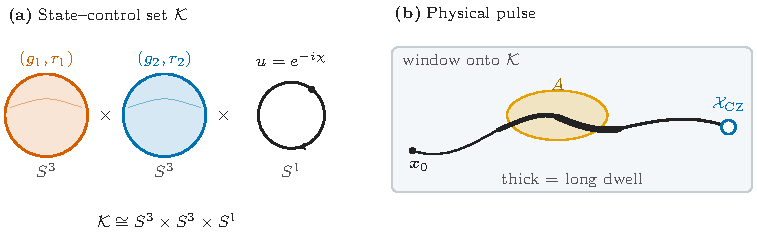
\includegraphics[width=0.88\textwidth]{figures/fig_occupation.pdf}
\caption{Geometry of the active-time
problem~\eqref{eq:state_set}--\eqref{eq:exposure}.
(a)~$\mathcal K$ is the product of the two-sector state space $\mathcal{X}$,
whose coordinates $(g_k,r_k)$ are the ground and Rydberg amplitudes of sector
$k\in\{1,2\}$, and the unit circle of the drive $u=\ee^{-\ii\chi}$.
(b)~A pulse traces a curve $s\mapsto(\xv(s),u(s))$ in $\mathcal K$ from the
computational ground state $\xv_0=(1,0,1,0)$ to the CZ terminal orbit
$\mathcal{X}_{\mathrm{CZ}}$, a circle of global phase.
The later lower-bound constraints of~\eqref{eq:pop} live on these same two
sets, including patches such as $A$ that a given pulse never visits, so a
single pair $(V,n)$ bounds every pulse at once.}
\label{fig:occupation}
\end{figure*}

The two normalizations, the constraint $|u|^2=1$, and the CZ conditions are
polynomial equations in the real and imaginary parts of the amplitudes
$g_k,r_k$ and of the drive $u$; $\mathcal K$ is bounded. The unknowns are then
a unit-modulus pulse $u(s)$, a duration $S$, and a trajectory $\xv(s)$ that
obeys the stacked Schrödinger equation. The active-time problem is
\begin{equation}
\begin{aligned}
C_* \;:=\; \inf_{u(\cdot),\,S,\,\xv(\cdot)}
& \quad C[u]=\int_0^S c\bigl(\xv(s)\bigr)\,\dd s \\
\text{subject to:}
& \quad \dd \xv/\dd s = f\bigl(\xv(s),u(s)\bigr), \quad 0\le s\le S, \\
& \quad \xv(0)=\xv_0=(1,0,1,0), \\
& \quad \bigl(\xv(s),u(s)\bigr)\in\mathcal K \quad \text{for all } s, \\
& \quad \xv(S)\in\mathcal{X}_{\mathrm{CZ}}, \\
& \quad S<\infty.
\end{aligned}
\label{eq:exposure}
\end{equation}
Every ingredient of~\eqref{eq:exposure} is a polynomial, or is the solution
set of polynomial equations; the next paragraph exploits that structure.

A lower bound on $C_*$ is a number that does not exceed $C[u]$ for every
admissible pulse. That number is a conservative estimate, at the initial state
$\xv_0$, of the exposure still owed to finish a CZ. Write $W(\xv)$ for such an
estimate at a general state $\xv$. On the terminal orbit the gate is already
done, so
\begin{equation}
W(\xv)\le 0 \qquad\text{for all }\xv\in\mathcal{X}_{\mathrm{CZ}}.
\label{eq:W_term}
\end{equation}
Along any trajectory $W$ cannot fall faster than the running cost is paid,
\begin{equation}
\frac{\dd W}{\dd s}\ge -c.
\label{eq:W_drift}
\end{equation}
Integrating from $\xv_0$ to $\xv(S)$ then gives $C[u]\ge W(\xv_0)$. We realize $W$ as
$W=-n-V$, with $n$ a real shift and $V$ a real polynomial in the real and
imaginary parts of $\xv$. Because $\dd W/\dd s=-\nabla V\cdot f$,
condition~\eqref{eq:W_term} is $p_{\mathrm{term}}\ge0$ and
condition~\eqref{eq:W_drift} is $p_{\mathrm{drift}}\ge0$, where
\begin{equation}
\begin{gathered}
p_{\mathrm{drift}}(\xv,u):=c(\xv)-\nabla V(\xv)\cdot f(\xv,u),\\
p_{\mathrm{term}}(\xv):=V(\xv)+n,
\end{gathered}
\label{eq:barrier_polys}
\end{equation}
where $\nabla V\cdot f$ is the directional derivative of $V$ along $f(\xv,u)$.
Because $V$ and $f$ are polynomials, so is $p_{\mathrm{drift}}$. We call
$p_{\mathrm{drift}}\ge0$ on $\mathcal K$ the drift inequality and
$p_{\mathrm{term}}\ge0$ on $\mathcal{X}_{\mathrm{CZ}}$ the terminal inequality.

The bound $C[u]\ge W(\xv_0)=-n-V(\xv_0)$ already holds for every admissible pulse.
What remains is to search over a polynomial $V$ of degree at most $D$ and the
shift $n$. The best such bound is the value of
\begin{equation}
\begin{aligned}
\sup_{V,\,n}
& \quad W(\xv_0)=-n-V(\xv_0) \\
\text{subject to:}
& \quad \deg V\le D,\quad n\in\mathbb{R}, \\
& \quad p_{\mathrm{drift}}(\xv,u)\ge0\quad\text{for all }(\xv,u)\in\mathcal K, \\
& \quad p_{\mathrm{term}}(\xv)\ge0\quad\text{for all }\xv\in\mathcal{X}_{\mathrm{CZ}}.
\end{aligned}
\label{eq:pop}
\end{equation}
This is an optimization problem in the coefficients of $V$ and the scalar $n$.
The symbols $g_k$, $r_k$, and $u$ are complex indeterminates with independent
conjugates, not real state variables and not unknowns of the program. The
duration $S$ is not an unknown, so any feasible pair $(V,n)$ bounds every
finite pulse at once (Fig.~\ref{fig:occupation}). The two inequalities are not
a finite list of polynomial constraints, so a solver cannot take~\eqref{eq:pop}
as written.

A sufficient, finite replacement uses the defining equations of the two sets as
rewrite rules. On $\mathcal K$,
\begin{equation*}
\bar u\,u=1,\qquad \bar g_k g_k=1-\bar r_k r_k\quad (k=1,2).
\end{equation*}
After these substitutions a monomial never carries a
simultaneous barred and unbarred power of $u$, $g_1$, or $g_2$.
Let $z$ be the finite column of all such monomials of total degree at
most $d$. On $\mathcal{X}_{\mathrm{CZ}}$ impose the same two normalizations and
then
\begin{equation*}
r_1=r_2=0,\qquad g_2=-g_1^2.
\end{equation*}
Let $w$ be the finite column of the surviving monomials in $g_1,\bar g_1$ of
degree at most $d$. The columns $z$ and $w$ assemble the sum-of-squares
certificates; $V$ itself is a real-valued polynomial in the reduced state
monomials (no $u$). A polynomial is a sum of squares in this monomial basis when
it equals $z^*Qz$ (resp.\ $w^*Qw$) with a real symmetric
Gram matrix $Q\succeq0$. Equating coefficients of like monomials is a finite
list of linear equalities. The unknowns are the coefficients of $V$, the
scalar $n$, and two such Gram matrices. The terminal identity constrains only
the restriction of $V+n$ to the CZ orbit; the objective uses the unrestricted
polynomial at $\xv_0$. The resulting semidefinite program is
\begin{equation}
\begin{aligned}
\sup_{V,\,n,\,Q}
& \quad -n-V(\xv_0) \\
\text{subject to:}
& \quad p_{\mathrm{drift}}
\equiv z^*Q_{\mathrm{drift}}z
\quad (\mathcal K), \\
& \quad Q_{\mathrm{drift}}\succeq0, \\
& \quad p_{\mathrm{term}}
\equiv w^*Q_{\mathrm{term}}w
\quad (\mathcal{X}_{\mathrm{CZ}}), \\
& \quad Q_{\mathrm{term}}\succeq0.
\end{aligned}
\label{eq:sdp}
\end{equation}
This is the program we solve~\cite{Lasserre01,Parrilo03,Putinar93}. Any
feasible point of~\eqref{eq:sdp} is feasible for~\eqref{eq:pop}. The order $d$
fixes the length of $z$ and $w$ and hence the degree of $V$; at the order $6$
used in Sec.~\ref{sec:split_exact}, $\deg V\le 2d-1=11$. Program~\eqref{eq:sdp}
is finite, but those columns grow rapidly with $d$, and a single pair $(V,n)$
on all of $\mathcal{K}$ still yields only a coarse underestimate of $C_*$.

% =========================================================================
\subsection{Symmetry reduction of the unsplit program}
\label{sec:sos_reductions}
% =========================================================================

The columns of~\eqref{eq:sdp} grow rapidly with $d$. Before raising the
order we shrink them by symmetry. Three maps preserve $f$, $c$,
$\mathcal K$, and $\mathcal{X}_{\mathrm{CZ}}$. A constant optical-phase
offset of the drive $u$ can be absorbed into the phase convention of the
Rydberg amplitudes, $u\mapsto\ee^{\ii\theta}u$ and
$r_k\mapsto\ee^{-\ii\theta}r_k$ with $g_k$ held fixed (optical gauge, or
laser-phase rotation). A local $Z$ that co-phases $\bket{r}$ with
$\bket{1}$ phases the one-atom sector once and the two-atom sector twice,
$(g_1,r_1)\mapsto\ee^{\ii\alpha}(g_1,r_1)$ and
$(g_2,r_2)\mapsto\ee^{2\ii\alpha}(g_2,r_2)$, with the same weight as the
CZ condition $g_2=-g_1^2$ (qubit gauge). Complex conjugation together
with $u\mapsto-\bar u$ (a $\pi$ flip of the laser phase $\chi$) is a
forward-time symmetry of the drive, acting as $u\mapsto-\bar u$,
$g_k\mapsto\bar g_k$, and $r_k\mapsto\bar r_k$ (combined reflection).
Figure~\ref{fig:symmetry}(a) records these three maps.

We restrict $(V,n)$ to pairs invariant under
the laser-phase and qubit-gauge rotations.
Invariance of $f$, $c$, $\mathcal K$, and $\mathcal{X}_{\mathrm{CZ}}$
keeps every such pair feasible for~\eqref{eq:pop}. Each variable then acquires a
definite phase $\ee^{\ii q\cdot(\theta,\alpha)}$; the integer pair $q$ is
its charge, $q(u)=(1,0)$, $q(g_1)=(0,1)$, $q(r_1)=(-1,1)$,
$q(g_2)=(0,2)$, $q(r_2)=(-1,2)$. A monomial $\bar z^\alpha z^\beta$ picks
up $\ee^{\ii(q(\beta)-q(\alpha))\cdot(\theta,\alpha)}$ and is invariant
only when $q(\alpha)=q(\beta)$. The Gram matrices of~\eqref{eq:sdp}
cannot mix two monomials of different charge and therefore split into one
positive-semidefinite block per charge: at unsplit order~$6$ that is
$113$ real blocks, the largest $75\times75$
(Fig.~\ref{fig:symmetry}(b); Appendix Table~\ref{tab:sos_progression}).
Invariant sums of squares yield that block
structure~\cite{Gatermann04,Riener13}. The remaining $\mathbb{Z}_2$
(reflection) does not split the blocks further; reflection rephasing
multiplies representatives of odd degree in $u$ by $\ii$, an
invertible change of basis that makes each block real symmetric without
changing the represented polynomial.

\begin{figure*}[t]
\centering
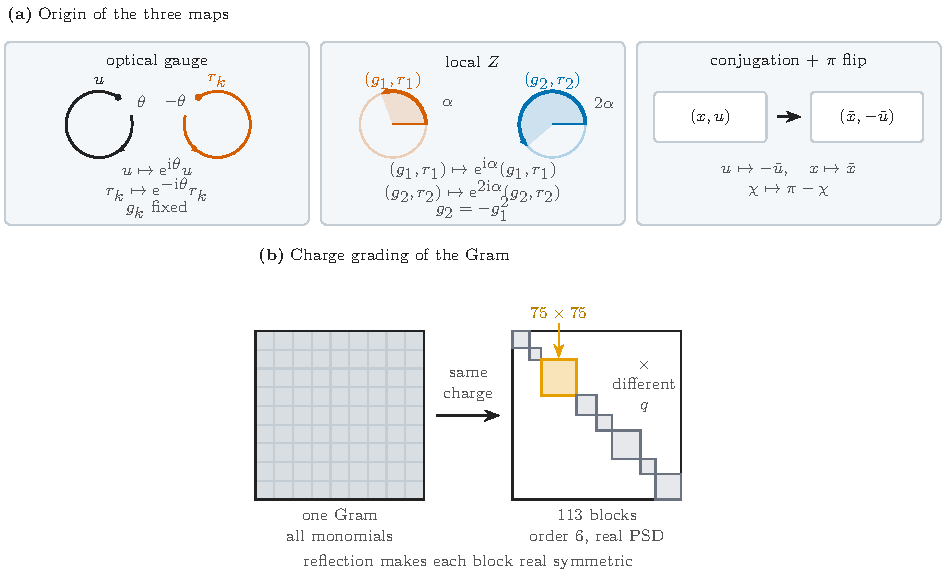
\includegraphics[width=0.92\textwidth]{figures/fig_symmetry.pdf}
\caption{The two $U(1)$ symmetries of
$(f,c,\mathcal K,\mathcal{X}_{\mathrm{CZ}})$ grade the monomials by
charge, so each sum-of-squares Gram of the order-$6$
program~\eqref{eq:sdp} is block-diagonal: $113$ real
positive-semidefinite blocks, the largest $75\times75$ (Appendix
Table~\ref{tab:sos_progression}). (a)~The three maps: optical gauge
(laser-phase rotation); local $Z$ with $\bket{r}$ co-phased (qubit
gauge) with weight~$2$ on the two-atom sector; and complex conjugation
together with a $\pi$ flip of the laser phase $\chi$. (b)~After charge
grading the Gram splits into
those blocks; reflection rephasing makes each block real symmetric
without changing the represented polynomial.}
\label{fig:symmetry}
\end{figure*}

Even after this reduction, a single pair $(V,n)$ on all of $\mathcal K$ stalls.
Floating solutions of~\eqref{eq:sdp} rise only from $2.8625$ at $d=6$ to
$2.9047$ at $d=11$, remaining $0.031$ below the certified ceiling
$C_{\mathrm{up}}=2.935875225844105$ of Sec.~\ref{sec:interval_closure}. Among
the unsplit hierarchy, only the order-$8$ solution was made exact, yielding
$C_*\ge1153/400=2.8825$; the floating objectives at $d\ge9$ are not bounds.
Across that range the largest PSD block grows
from $75$ to $758$ and the number of PSD entries from $54{,}078$ to
$13{,}916{,}543$ (Appendix Table~\ref{tab:sos_progression}), so raising $d$
further is prohibitive. A single low-degree polynomial $V(\xv)$ on all of $\mathcal K$ remains a coarse underestimate: near $r_k\approx0$ the
instantaneous cost is small, so the remaining-exposure estimate can hardly fall, yet it must still drop by the full bound between $\xv_0$ and the CZ orbit. Symmetry shrinks~\eqref{eq:sdp}
at fixed $d$ but does not enlarge what a polynomial in $\xv$ can express. The next subsection
supplies a second argument.

% =========================================================================
\subsection{Cumulative-exposure partition}
\label{sec:exposure_partition}
% =========================================================================

The unsplit hierarchy of Sec.~\ref{sec:sos_reductions} improves toward
$C_*$ only at high polynomial order. The remaining exposure is a function of $\xv$ alone; the obstruction is representational.
We do not raise the degree. We introduce a second argument,
the budget coordinate $X$: the fraction of a known exposure ceiling $U$
already spent. A low-degree function of $(X,\xv)$, cut into cells, can tighten the underestimate at accessible order.

That ceiling is not a new constraint on the laser.
Sec.~\ref{sec:interval_closure} certifies an exact CZ gate with
$C_*<C_{\mathrm{up}}$ by interval arithmetic, below the rational ceiling
$U:=2935887/1000000$ ($C_{\mathrm{up}}<U$). Pulses with $C[u]\ge U$ already
lose to that gate and may be ignored. For every remaining pulse, $U$ is a
ceiling and
\begin{equation}
X(s):=\frac1U\int_0^s c\bigl(\xv(s')\bigr)\,\dd s'\in[0,1)
\label{eq:exposure_odometer}
\end{equation}
records the paid fraction of that ceiling. The budget starts at $X=0$ and
approaches $1$ when the pulse has almost paid $U$. It is not laboratory
time and not progress toward the CZ target: a pulse that dwells in Rydberg
states without approaching the gate still advances it. A Putinar
sum-of-squares representation requires a compact constraint
set~\cite{Putinar93}. The active time $s$ is unbounded, so that
hypothesis fails and a polynomial in $s$ cannot serve as a uniform
second argument.

A single low-degree polynomial in $(X,\xv)$ would still have to cover the
whole bill. The hard stretches are the two ends. Just after leaving
$\xv_0$ one has $X\approx0$ and $r_k\approx0$: the remaining-exposure
estimate must stay large, yet the instantaneous cost is small, so the
estimate may hardly fall. Just before arrival on the CZ set one has $X$
near $1$ and $r_k\approx0$ again: the estimate must already be near
zero, and again it may hardly fall. The two ends are both cheap, yet the estimate must differ by the full bound between them; one low-degree polynomial on the whole bill is what stalls. We
therefore cut $[0,1]$ at rational knots and give each stretch its own
polynomial. The budget only increases, so every pulse crosses the cells
from left to right. Cell $j$ has width $w_j$ and a local coordinate
$\xi_j\in[0,1]$,
\begin{equation}
\begin{gathered}
0=a_0<a_1<\cdots<a_J=1,\\
w_j=a_j-a_{j-1},\qquad\xi_j=\frac{X-a_{j-1}}{w_j}.
\end{gathered}
\label{eq:split_grid}
\end{equation}
On that cell $\xi=0$ at the left knot and $\xi=1$ at the right knot:
$\xi$ is the fraction of this stretch already spent, not a new time.
The remaining-exposure estimate is a polynomial
$W_j(\xi,\xv)=-n-V_j(\xi,\xv)$, with the same shift $n$ as in
Sec.~\ref{sec:occupation}.

As in Sec.~\ref{sec:occupation}, the estimate cannot fall faster than
the pulse pays. The polynomial $V_j$ now depends on $\xi$ as well as on
$\xv$, and $\xi$ advances only while the atoms occupy Rydberg states,
$\dd\xi_j/\dd s=c(\xv)/(Uw_j)$. The chain rule therefore adds one term to
the directional derivative of Sec.~\ref{sec:occupation}. The drift
polynomial is
\begin{equation}
\begin{gathered}
p_{\mathrm{drift},j}
:=c-\nabla_{\xv} V_j\cdot f-\frac{c}{Uw_j}\,\partial_\xi V_j,\\
L_j:=f\cdot\nabla_{\xv}+\frac{c}{Uw_j}\,\partial_\xi,
\end{gathered}
\label{eq:split_generator_mass}
\end{equation}
with $p_{\mathrm{drift},j}=c-L_jV_j$. The drift inequality is
$p_{\mathrm{drift},j}\ge0$ on $[0,1]\times\mathcal K$. When the pulse
crosses a knot it pays nothing extra, so the remaining-exposure
estimate cannot jump down, $W_j(1,\xv)\le W_{j+1}(0,\xv)$, or equivalently
$V_j(1,\xv)\ge V_{j+1}(0,\xv)$ on $\mathcal{X}$; otherwise the stretches
would not add. On the CZ set the estimate is still nonpositive,
$W_j\le0$. The program at degree $D$ is therefore
\begin{equation}
\begin{aligned}
\sup_{V_1,\dots,V_J,\,n}
& \quad W_1(0,\xv_0)=-n-V_1(0,\xv_0) \\
\text{subject to:}
& \quad \deg V_j\le D,\quad n\in\mathbb{R}, \\
& \quad p_{\mathrm{drift},j}(\xi,\xv)\ge0
\quad\text{on }[0,1]\times\mathcal K,\\
& \quad\qquad j=1,\dots,J, \\
& \quad V_j(1,\xv)-V_{j+1}(0,\xv)\ge0
\quad\text{on }\mathcal{X},\\
& \quad\qquad j=1,\dots,J-1, \\
& \quad V_j(\xi,\xv)+n\ge0
\quad\text{on }[0,1]\times\mathcal{X}_{\mathrm{CZ}},\\
& \quad\qquad j=1,\dots,J.
\end{aligned}
\label{eq:split_pop}
\end{equation}

Each constraint is again a polynomial nonnegativity demand on a polynomially
defined set, now with $0\le\xi\le1$, so the finite replacement~\eqref{eq:sdp}
applies cell by cell with the extra multiplier $\xi(1-\xi)$. The charge
reduction of Sec.~\ref{sec:sos_reductions} applies cell by cell; the cones
are recorded in Appendix~\ref{app:split_certificate}. A feasible point bounds
$C_*$ by the same chain-rule argument as in Sec.~\ref{sec:occupation};
Theorem~\ref{thm:split_exact} writes the telescope.

The primary certificate uses the five-cell grid
\begin{equation}
(a_0,\ldots,a_5)=\left(0,\frac1{26},\frac13,\frac23,\frac{25}{26},1\right),
\label{eq:primary_split_grid}
\end{equation}
The two narrow end cells $[0,1/26]$ and $[25/26,1]$ give a full local
coordinate $\xi$ to those short, cheap stretches; the middle cells are
wider, where the cost is of order one and $\xv$ already distinguishes the
state. A finer partition enlarges the program without tightening the
bound: at the same order the six-cell value is still $2.930$
(Table~\ref{tab:sos_comparison}). Order~$6$ on this grid reaches
$2.930$. The next subsection replaces a floating solution
of~\eqref{eq:split_pop} by an exact certificate.

\begin{table}[t]
\centering
\caption{Convergence of moment-SOS lower bounds under unsplit and cumulative-exposure-split formulations. Starred ($\ast$) entries are exact algebraic dual certificates over $\mathbb{Q}(\sqrt{2})$. The daggered ($\dagger$) entry denotes the exact physical-slack extension built upon the order-$7$ dual certificate; it is not a direct SDP optimum. Unsplit solver dimensions appear in Appendix Table~\ref{tab:sos_progression}; the baseline five-cell certificate is audited through $9{,}180$ identities and $2{,}665$ Gram blocks (Appendix~\ref{app:auditor}).}
\label{tab:sos_comparison}
\vspace{0.3em}
\footnotesize
\resizebox{\columnwidth}{!}{%
\begin{tabular}{@{}lcccc@{}}
\toprule
Formulation & Order $d$ & Domain partition & Lower bound & Gap to $C_{\mathrm{up}}$ \\
\midrule
Unsplit & 6  & --- & $2.8625$ & $0.0734$ \\
Unsplit & 8  & --- & $2.8825^\ast$ & $0.0534$ \\
Unsplit & 11 & --- & $2.9047$ & $0.0311$ \\
\midrule
Split & 7 & 3-cell & $2.9250^\ast$ & $0.0109$ \\
Split & 6 & 5-cell & $2.9300^\ast$ & $0.0059$ \\
Split & 6 & 6-cell & $2.9300^\ast$ & $0.0059$ \\
Split & 7 & 5-cell & $2.9305^\ast$ & $0.0054$ \\
Slack extension & 7 (base) & 5-cell & $\mathbf{2.931287735220}^\dagger$ & $\mathbf{0.004587}$ \\
\bottomrule
\end{tabular}%
}
\end{table}

% =========================================================================
\subsection{Exact certificate over \texorpdfstring{$\mathbb{Q}(\sqrt{2})$}{Q(sqrt(2))}}
\label{sec:split_exact}
% =========================================================================

The drift polynomial~\eqref{eq:split_generator_mass} contains the vector
field~\eqref{eq:vector_field},
\begin{equation}
\begin{gathered}
L_jV_j
= f\cdot\nabla_{\xv} V_j+\frac{c(\xv)}{Uw_j}\,\partial_\xi V_j,\\
f=-\frac{\ii}{2}\bigl(u\,r_1,\ \bar u\,g_1,\ \sqrt2\,u\,r_2,\ \sqrt2\,\bar u\,g_2\bigr).
\end{gathered}
\label{eq:Lj_sqrt2}
\end{equation}
The two-atom components inject $\sqrt{2}$ into every drift polynomial
$c-L_jV_j$. The remaining data of~\eqref{eq:split_pop}, namely $c$ and the
cell widths $Uw_j$, are rational. The certificate constructed and verified below has coefficients in
that same field:
\begin{equation}
V_j(\xi,\xv)
=\sum_{\alpha}\bigl(a_{j\alpha}+b_{j\alpha}\sqrt{2}\bigr)\,m_{\alpha}(\xi,\xv),
\qquad a_{j\alpha},b_{j\alpha}\in\mathbb{Q}.
\label{eq:Vj_qsqrt2}
\end{equation}
Numerical semidefinite programs supply floating-point seeds for those
coefficients, the scalar $n$, and the Gram matrices. We reconstruct them
exactly in the quadratic field
$\mathbb{Q}(\sqrt{2})=\{a+b\sqrt{2}:a,b\in\mathbb{Q}\}$ and certify every Gram
matrix positive semidefinite by a rational $\mathrm{LDL}^{\mathsf T}$
factorization~\cite{Peyrl08,Rump06}. Exact arithmetic removes solver tolerance
from the proof.

Table~\ref{tab:sos_comparison} shows that the order-$6$ five-cell program reaches
$C_*\ge2.930$. It improves on the order-$11$ unsplit program while concentrating
polynomial degree on the two narrow end cells.

\begin{theorem}[Exact five-cell split dual]
\label{thm:split_exact}
Under the hypotheses of Lemma~\ref{lem:bang}, the physical amplitude-limited CZ exposure infimum satisfies
\begin{equation}
C_* \;\ge\; \frac{293}{100} \;=\; 2.930.
\label{eq:split_bound}
\end{equation}
\end{theorem}
\begin{proof}
Fix any competitive trajectory with $C<U$ and the five-cell
partition~\eqref{eq:primary_split_grid}. Let $j_*$ be the cell that contains
$X(S)\in[0,1)$, and write $0=s_0<\cdots<s_{j_*-1}<s_{j_*}=S$ for the active times
at which the trajectory crosses the interfaces $X=a_j$ for $j<j_*$. The exact
certificate supplies a feasible point of~\eqref{eq:split_pop}: real polynomials
$V_1,\ldots,V_5$ of degree at most $11$ and a scalar $n\in\mathbb{Q}(\sqrt{2})$
such that $c-L_jV_j\ge0$ throughout each cell, $V_j(1,\cdot)\ge V_{j+1}(0,\cdot)$
at every interface, and $V_j+n\ge0$ on the terminal orbit
(Appendix~\ref{app:terminal_quotient}). Integrating $\dd V_j/\dd s=L_jV_j\le c(\xv)$
along each traversed segment and summing yields
\begin{equation}
\begin{aligned}
C
&=\sum_{j=1}^{j_*-1}\int_{s_{j-1}}^{s_j}c\bigl(\xv(s)\bigr)\,\dd s
+\int_{s_{j_*-1}}^{S}c\bigl(\xv(s)\bigr)\,\dd s\\
&\ge\sum_{j=1}^{j_*-1}\Bigl[V_j\bigl(1,\xv(s_j)\bigr)-V_j\bigl(0,\xv(s_{j-1})\bigr)\Bigr]\\
&\qquad+\Bigl[V_{j_*}\bigl(\xi(S),\xv(S)\bigr)-V_{j_*}\bigl(0,\xv(s_{j_*-1})\bigr)\Bigr]\\
&\ge V_{j_*}\bigl(\xi(S),\xv(S)\bigr)-V_1(0,\xv_0)
\ge -n-V_1(0,\xv_0)
=\frac{293}{100}.
\end{aligned}
\label{eq:split_weak_duality}
\end{equation}
Exact nonnegativity of $c-L_jV_j$, of the interface jumps
$V_j(1,\cdot)-V_{j+1}(0,\cdot)$, and of the terminal polynomials $V_j+n$ on
$\mathcal{X}_{\mathrm{CZ}}$ is verified in the form~\eqref{eq:sdp}
with sums of squares in $\mathbb{Q}(\sqrt{2})$, through $9{,}180$ coefficient
identities and $2{,}665$ Gram blocks, without floating-point tolerances
(Appendix~\ref{app:auditor}; constraint cones in
Appendix~\ref{app:split_certificate}). Trajectories with $C\ge U>293/100$ satisfy
the bound automatically; Lemma~\ref{lem:bang} extends it to every
amplitude-limited laboratory pulse.
\end{proof}

An independent six-cell verification over $\mathbb{Q}(\sqrt{2})$, on the grid
$(0,1/26,1/4,1/2,3/4,25/26,1)$, recovers the same bound $C_*\ge293/100$.
Partitioning the cumulative-cost coordinate resolves the endpoints more
efficiently than raising a single global degree (Table~\ref{tab:sos_comparison}).
While this order-$6$ certificate provides a self-contained algebraic baseline at $C_* \ge 2.930$, refining the split program to order $7$ on the grid $(0, 1/36, 1/3, 2/3, 35/36, 1)$ raises the direct SDP dual bound to $L = 5861/2000 = 2.9305$ (Table~\ref{tab:sos_comparison}). Because the SDP dual evaluates the worst-case bound over formal measures that may visit dynamically unphysical regions, it leaves residual conservatism. Rather than pursuing computationally prohibitive higher polynomial degrees, one can capture unavoidable positive slack along physical trajectories, leading to the strengthened lower bound below.

\begin{theorem}[Slack-strengthened certified lower bound]
\label{thm:slack_strengthened}
Under the hypotheses of Lemma~\ref{lem:bang}, the physical amplitude-limited CZ exposure infimum satisfies
\begin{equation}
C_* \;\ge\; \frac{146564386761}{50000000000} \;=\; 2.931287735220.
\label{eq:slack_strengthened_bound}
\end{equation}
\end{theorem}
\begin{proof}
The order-$7$, five-cell split dual certificate on the grid $(0, 1/36, 1/3, 2/3, 35/36, 1)$ first yields an exact baseline decomposition $C[u] - L \ge 0$ with $L = 5861/2000 = 2.9305$, expressed as a sum of nonnegative occupation, interface, and terminal terms. A supplementary certificate then proves that along every physical CZ trajectory, this excess is strictly bounded away from zero. In particular, the dark-state coordinate $D = g_1r_2 - \sqrt{2}g_2r_1$ obeys the dynamical speed limit $|D'| \le c/\sqrt{2}$ with running cost $c = |r_1|^2/2 + |r_2|^2/4$. Since $r_1=r_2=0$ at both initial and final times, integrating $|D'|$ from either boundary enforces $|D(s)| \le \min(C(s), C_{\mathrm{tot}}-C(s))/\sqrt{2}$, where $C(s)$ is the accumulated exposure and $C_{\mathrm{tot}}$ is the total pulse cost. This dynamical barrier excludes large regions of the population space $(|r_1|^2, |r_2|^2)$ from being reachable. Under the contradiction hypothesis $C_{\mathrm{tot}} < 146564386761/50000000000$, the credited slack across reachable cells and mandatory interface crossings strictly exceeds $C_{\mathrm{tot}} - L$. The resulting degree-$13$ terminal polynomial has $14$ Bernstein coefficients that are all strictly positive in exact rational arithmetic. Thus, no physical trajectory can close the gate below the stated threshold.
\end{proof}

We emphasize that the value $2.931287735220$ is not a rounded floating-point optimum or a heuristic rational reconstruction. The proof operates in two rigorous tiers: the direct algebraic SDP establishes $L = 2.9305$, and the supplementary checker establishes strictly positive slack by integrating physical conservation laws and state-space reachability exclusions under per-Gram budget constraints. All coefficient identities and the terminal Bernstein positivity are verified in exact rational arithmetic over $\mathbb{Q}$, independent of solver precision or numerical sampling.

\section{Certified upper bound and optimal pulse dynamics}
\label{sec:pulse}
% =========================================================================

While the moment-SOS dual certificate and its physical-slack extension prove $C_* \ge 2.9313$ for all globally driven CZ gates, a matching existence proof is still required to turn a numerical candidate into an unconditional upper bound. In this section we certify by interval arithmetic~\cite{Johansson17} that an exact CZ gate exists with exposure strictly below $2.935875225844105$ (Sec.~\ref{sec:interval_closure}). The certified $12{,}672$-segment witness is too finely resolved to display the mechanism. We therefore inspect a compact $192$-segment waveform in the same low-exposure regime and map the duration--exposure trade-off that shapes it (Sec.~\ref{sec:exposure_dynamics}).

\subsection{Interval-certified gate closure}
\label{sec:interval_closure}
Any admissible pulse that realizes an exact CZ gate supplies an upper bound on $C_*$. Floating-point ordinary differential equation (ODE) integrations, however, leave terminal residuals of order $10^{-16}$--$10^{-6}$ together with discretization artifacts, so a numerical candidate alone cannot certify a mathematical ceiling. We therefore construct a computer-assisted existence proof: interval arithmetic and the Krawczyk fixed-point theorem~\cite{Krawczyk69} eliminate all floating-point and discretization residual errors and certify an exact, zero-residual CZ root.

The witness is a piecewise-constant phase pulse of $12{,}672$ equal-duration segments at active time $S\approx7.739116$. Unitarity together with the CZ target~\eqref{eq:CZ_cond} amounts to five real terminal conditions. The pulse family is far larger than five-dimensional, so those conditions do not select a unique waveform. We therefore restrict the residual map $F$ to one regular five-parameter slice of the family, refine that square system by multi-precision Newton until $\lvert F\rvert<10^{-135}$, and apply the Krawczyk test to the resulting $\mathbb{R}^5\to\mathbb{R}^5$ map~\cite{Krawczyk69}. The slice, the components of $F$, and the contraction estimates are recorded in Appendix~\ref{sec:interval_methods}.

Evaluating the segment propagators in $500$-bit Arb interval arithmetic~\cite{Johansson17} over a box of radius $10^{-80}$ about the refined candidate shows that the Krawczyk image of the box lies strictly inside the box~\cite{Krawczyk69}. That inclusion proves $F$ has a unique exact root in the box. On this same box one also has $\operatorname{Re}(g_2\bar g_1^2)<0$, so the root is an entangling CZ gate rather than a trivial identity cycle. The operator and the contraction estimates are in Appendix~\ref{sec:interval_methods}. Integrating the exposure over the certified box produces
\begin{equation}
C_* < C_{\mathrm{up}} := 2.935875225844105.
\label{eq:upper_bound}
\end{equation}
The certified exposure interval has radius $5.06\times10^{-79}$ about $2.9358752258441048994\ldots$, so the strict inequality holds against the rounded upper endpoint and confirms that an admissible exact CZ trajectory exists below this ceiling.

\subsection{Trajectory dynamics and duration-dependent exposure}
\label{sec:exposure_dynamics}
Figure~\ref{fig:pulse} shows an optimized $192$-segment waveform at $S=7.725$ ($C\approx2.9360$), in the same low-exposure regime as Locher \emph{et al.}~\cite{Locher25}.

Population desynchronization is the first structural signature. Generating a net nonlocal phase $\zeta:=\arg g_2-2\arg g_1$ requires a stretch of time with nonzero synchronization error $w:=z_2-\sqrt{2}z_1$, where $z_k=r_k/g_k$ (Appendix~\ref{app:coordinates}, Lemma~\ref{lem:ratio}). The population traces in Fig.~\ref{fig:pulse}(a) are one realization of that desynchronization: the single-excitation population $p_1=|r_1|^2$ rises rapidly into a broad central plateau that sustains continuous ground-state phase accumulation $\Phi_1=\arg g_1$, while the collective population $p_2=|r_2|^2$ reaches a local minimum near $0.45$ at the midpoint $s=S/2$. The collective sector evolves at a $\sqrt{2}$-enhanced Rabi rate and therefore completes more of its phase excursion earlier; lowering $p_2$ in the central window cuts two-atom Rydberg decay while the slower single-excitation sector finishes accumulating $\Phi_1$. Both sectors then return to the computational manifold together at $s=S$.

A second signature is visible in Fig.~\ref{fig:pulse}(b): the unwrapped laser phase $\chi(s)$ is antisymmetric about $s=S/2$, although that symmetry was not imposed on the search. The outbound half of the pulse then retraces the inbound half in reverse.

The continuous nonlocal phase $\zeta(s)$ records the geometric necessity of this orchestration [Fig.~\ref{fig:pulse}(c)]. It crosses $-\pi/2$ at the midpoint, overshoots to $-3.56$~rad ($-1.13\pi$) near $s\approx0.68S$, and only then settles smoothly onto the CZ target $-\pi$ at $s=S$. The overshoot is not an artifact of discretization: because $p_2$ has already been lowered, the remaining single-excitation steering temporarily drives $\zeta$ past $-\pi$; the final return of $p_1$ and the antisymmetric phase profile then pull $\zeta$ back to exact closure. A monotone march from $0$ to $-\pi$ cannot accommodate the midpoint dip while keeping both sectors closed.

The pulse at $S=7.725$ is one point on a broader duration--exposure scan of $96$-segment local-search candidates. Mapping those candidates across $S\in[7.612,16]$ with multi-start limited-memory Broyden--Fletcher--Goldfarb--Shanno (L-BFGS) followed by equality-constrained sequential least squares programming (SLSQP) on $96$-segment waveforms, together with a $192$-segment refinement at $S=7.725$ and a warm start at $S=16$ (Appendix~\ref{sec:methods}), reveals three regimes in that search. At the short-duration edge, searches encounter a numerical quantum speed limit (QSL) near $S\approx7.612$~\cite{JP22,Fromonteil24}, below which both sectors fail to close simultaneously. Operating on this boundary forces both state vectors through their loops at full capacity; the midpoint dip has no time to form, and the exposure rises to $C\approx2.9571$. Immediately beyond the cutoff, the candidates drop into a flat minimal-exposure basin spanning $S\in[7.7,8.5]$, with its floor near $S=7.725$ at $C\approx2.9360$ and less than $0.1\%$ variation across the basin. For still longer gates ($S>8.5$), the same $96$-segment local-search candidates drift upward.

\begin{figure}[t]
\centering
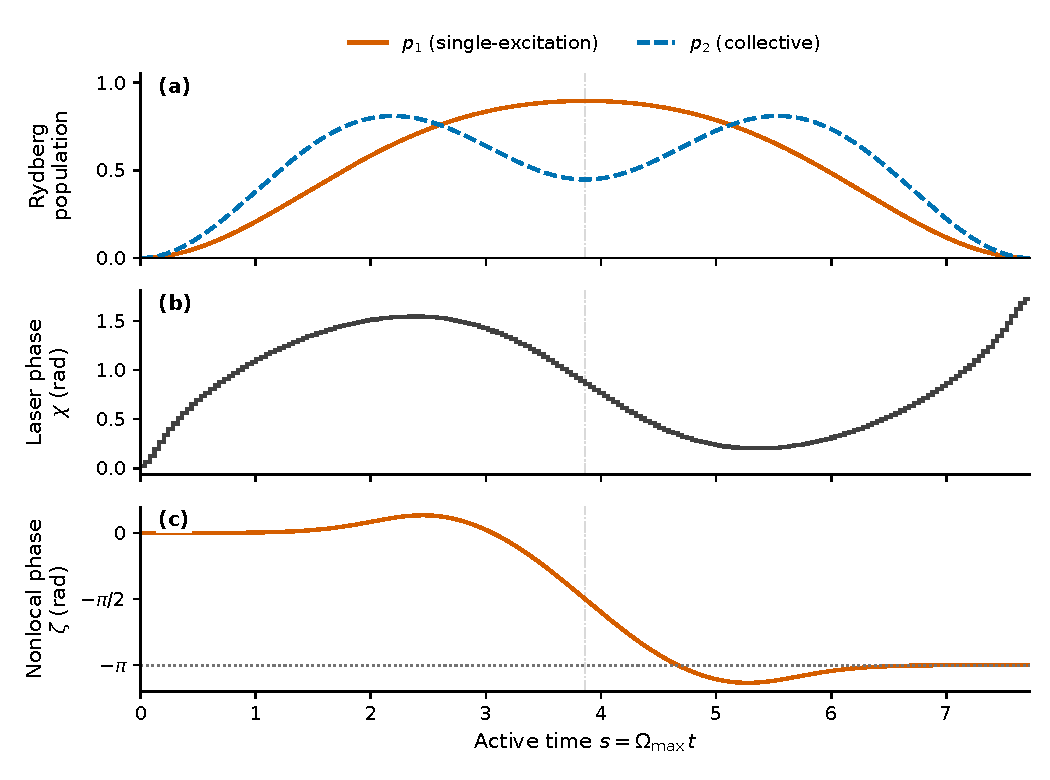
\includegraphics[width=\columnwidth]{figures/fig_pulse.pdf}
\caption{Dynamical mechanism of Rydberg exposure minimization for the archived $192$-segment waveform at duration $S=7.725$ ($C\approx2.935956$). (a)~Sector Rydberg populations $p_k=|r_k|^2$: the single-excitation population $p_1$ (solid) forms a broad plateau that sustains phase accumulation $\Phi_1$, while the collective population $p_2$ (dashed) reaches a local minimum near $0.45$ at the midpoint $s=S/2$ (dash-dotted vertical line), reducing two-atom decay before both sectors close at $s=S$. (b)~Unwrapped piecewise-constant laser phase $\chi(s)$, antisymmetric about the midpoint. (c)~Continuous nonlocal phase $\zeta(s)=\arg g_2-2\arg g_1$, which crosses $-\pi/2$ at the midpoint, overshoots to $-3.56$~rad ($-1.13\pi$) at $s\approx0.68S$, and closes at $-\pi$ (dotted horizontal line). Exact segment matrix exponentials give a floating closure residual of $4.4\times10^{-27}$.}
\label{fig:pulse}
\end{figure}

% =========================================================================
\section{Discussion and outlook}
\label{sec:discussion}
% =========================================================================

The duration--exposure candidates of Sec.~\ref{sec:exposure_dynamics} already sit against the certified window
\begin{equation}
2.9313 \le C_* < 2.9359,
\label{eq:certified_window_disc}
\end{equation}
of relative width $0.16\%$. Existing waveforms approach within $0.003\%$ of this certified ceiling, so the remaining laboratory question is not whether pulse shaping can still cut decay by a large factor, but how to spend duration against technical noise $\gamma T$.

\textit{Duration--exposure trade-off.---}The numerical speed-limit pulse ($S\approx7.612$, $C\approx2.9571$)~\cite{JP22} and the minimal-exposure pulse ($S=7.725$, $C\approx2.9360$)~\cite{Locher25} differ by a $0.71\%$ exposure cut at a $1.48\%$ longer duration. Under $1-\mathcal F\approx\Gamma\TR+\gamma T$, the longer pulse is preferable whenever
\begin{equation}
\frac{\gamma}{\Gamma} < \frac{2.9571 - 2.9360}{7.725 - 7.612} \approx 0.187.
\end{equation}
Long-lived, low-noise platforms therefore favor the $S=7.725$ basin; dephasing- or Doppler-limited ones favor the speed limit.

\textit{Erasure conversion.---}If instead $\gamma\ll\Gamma$, that choice collapses and the window is a floor: $\Gamma\TR\ge2.9313\,\Gamma/\Omax$. Converting Rydberg decay into detectable erasures~\cite{Wu22,Scholl23,Ma23} does not remove it. Even with ideal branching, the erasure probability cannot fall below $2.9313\,\Gamma/\Omax$.

\textit{Beyond a single global drive.---}Lowering exposure below $2.9313$ requires leaving the shared-drive model of Sec.~\ref{sec:model}. Dynamically, the floor arises because the single global field couples single- and two-excitation sectors at an incommensurate ratio; relaxing the dynamics to allow independent control over the two sectors removes this lock and drives the exposure infimum to zero (Theorem~\ref{thm:relax}). In physical architectures, independently addressing each atom with local laser beams does not decouple the sectors in this idealized way: the sequential gate of Jaksch \emph{et al.}~\cite{Jaksch00} incurs an exposure of $7\pi/4\approx5.50$, and whether continuous pulse shaping with site-resolved fields can undercut $2.9313$ remains an open question. Auxiliary dressing, dual-species control, and operation at finite blockade $B\sim\Omax$~\cite{DDP25} provide alternative routes. The leftover $0.16\%$ gap inside the present model may shrink with further analysis.

% =========================================================================
\clearpage
\onecolumngrid
\appendix

% =========================================================================
\section{No-go theorems for shortcut relaxations}
\label{sec:nogo}
% =========================================================================

This appendix proves two facts used in the main text. An isolated two-level atom can acquire any ground-state phase with exposure driven to zero. If the two excitation sectors also have independent controls, an exact CZ has the same vanishing infimum. Neither statement bounds the shared-drive $C_*$. Together they say that a strictly positive floor, if it exists, has to come from one laser locking both sectors, not from a per-sector phase condition and not from unlocking the drive.

The first fact is the following.
\begin{theorem}[A single two-level phase is free]
\label{thm:free}
For an uncoupled two-level system ($k=1$ or $2$) in active time with $|u|=1$ and unrestricted duration, the infimum of the exposure required to accumulate an arbitrary ground phase $\Phi$ with exact loop closure $r(S)=0$ is zero.
\end{theorem}
\begin{proof}
Let $m=1,2,\ldots$ index the successive returns of a constant-detuning drive to the ground state, $r=0$. Any target phase is already reachable at the first return $m=1$, but that exposure stays finite; sending $m\to\infty$ forces $|\Delta|$ to infinity and drives the exposure to zero. In units $\Omax=1$ with coupling $c=\sqrt{k}/2$, take the constant-detuning drive $\chi(s)=\Delta s$ ($|u|=1$). In the rotating frame $g=\tilde g\,\ee^{-\ii\chi/2}$, $r=\tilde r\,\ee^{\ii\chi/2}$, the dynamics~\eqref{eq:schrod} is autonomous with generator $H_{\mathrm{eff}}=\begin{pmatrix}-\Delta/2 & c\\ c & \Delta/2\end{pmatrix}$ and frequency $\omega=\sqrt{c^2+\Delta^2/4}$:
\begin{equation}
\tilde g(s)=\cos\omega s+\ii\frac{\Delta}{2\omega}\sin\omega s,
\qquad
\tilde r(s)=-\ii\,\frac{c}{\omega}\sin\omega s .
\end{equation}
At the loop times $S_m=m\pi/\omega$ the Rydberg amplitude closes exactly, $r(S_m)=0$, and $g(S_m)=(-1)^m\ee^{-\ii\Delta S_m/2}$, so the acquired phase is $\Phi_m=m\pi\bigl(1-\Delta/(2\omega)\bigr)\pmod{2\pi}$. The exposure is
\begin{equation}
E_m=\frac{c^2}{\omega^2}\int_0^{S_m}\sin^2\omega s\,\dd s=\frac{m\pi c^2}{2\omega^3}.
\end{equation}
The trivial target $\Phi=0\pmod{2\pi}$ is attained with zero exposure by the stationary control. For any nontrivial target, choose its representative $Q=\Phi/\pi\in(0,2)$. For fixed $m$, the map $\Delta\mapsto 1-\Delta/(2\omega)$ is continuous and strictly monotone with range $(0,2)$, so there is a unique $\Delta_m$ satisfying $1-\Delta_m/(2\omega_m)=Q/m$ and hence $\Phi_m=\Phi\pmod{2\pi}$. The $m=1$ choice already hits every phase, with finite exposure. For large $m$ one has $\Delta_m/(2\omega_m)=1-Q/m$, so $\omega_m^2=c^2\big/\bigl(1-[\Delta_m/(2\omega_m)]^2\bigr)=\Theta(m)$ and $\omega_m=\Theta(m^{1/2})$. The exposure then falls as
\begin{equation}
E_m=\frac{m\pi c^2}{2\omega_m^3}=\Theta(m^{-1/2})\xrightarrow[m\to\infty]{}0 .
\end{equation}
For a nontrivial target the infimum is zero but is not attained: $E=0$ would require $r\equiv 0$ almost everywhere, which freezes the phase. The required duration diverges, $S_m=\Theta(m^{1/2})$, which the unrestricted-duration problem permits.
\end{proof}

The second fact is the following.
\begin{theorem}[An unlocked CZ has exposure infimum zero]
\label{thm:relax}
If the two excitation sectors may be driven by independent bounded controls, the infimum of the exposure of an exact CZ is zero.
\end{theorem}
\begin{proof}
Give the collective sector its own drive $v_2$ and leave the single-excitation sector idle, $v_1\equiv 0$. Theorem~\ref{thm:free} then yields $\Phi_2=\pi$ with $r_2(S)=0$ and $E_2\to 0$, while $\Phi_1=0$ and $E_1=0$. The CZ condition $\Phi_2-2\Phi_1=\pi$ holds and the average exposure $(2E_1+E_2)/4\to 0$.
\end{proof}

% =========================================================================
\section{Analytical lower bound via a progress coordinate}
\label{sec:analytical}
% =========================================================================

The exposure $C=\int c\,\dd s$ is an integral along a pulse we do not know. Every exact CZ does, however, start in the computational ground states and return there with the CZ sign $g_2=-g_1^2$. In a shared three-level slot spanned by a $\bket{11}$-like amplitude, a $\bket{W}$-like amplitude, and a two-Rydberg amplitude, we place the physical blockaded collective spinor $A$ beside a companion $B$ built from the single-excitation dynamics as if the two atoms evolved independently with no blockade. Their overlap $z:=A^\dagger B$ equals $+1$ at the start and $-1$ at every such endpoint, so its real part $q=\operatorname{Re}z$ must travel from $+1$ to $-1$. The resulting analytical lower bound is $C_{\mathrm{fib}}$; it remains weaker than the global polynomial certificate of Sec.~\ref{sec:moments_sos}.

In that basis the third entry of $A$ vanishes, because perfect blockade forbids $\bket{rr}$. The companion $B$ is the symmetric square of $(g_1,r_1)$, so $\bket{rr}$ may be occupied, and $|g_1|^2+|r_1|^2=1$ implies $\|B\|=1$:
\begin{equation}
A(s) \;=\; \begin{pmatrix} g_2 \\ r_2 \\ 0 \end{pmatrix},
\qquad
B(s) \;=\; \begin{pmatrix} g_1^2 \\ \sqrt{2}g_1 r_1 \\ r_1^2 \end{pmatrix}.
\label{eq:AB_def}
\end{equation}
The laser couples $\bket{11}$ to $\bket{W}$ through the shared Hamiltonian $H_0$, which both $A$ and $B$ feel and which never reaches $\bket{rr}$ (its third row and column vanish). Blockade removes the additional $\bket{W}\leftrightarrow\bket{rr}$ coupling $H_1$ from the physical collective motion of $A$, while the companion $B$ still evolves under $H_0+H_1$ because it is constructed as if blockade were absent:
\begin{equation}
\begin{gathered}
H_0 = \frac{1}{\sqrt{2}}\begin{pmatrix} 0 & u & 0 \\ u^* & 0 & 0 \\ 0 & 0 & 0 \end{pmatrix},
\qquad
H_1 = \frac{1}{\sqrt{2}}\begin{pmatrix} 0 & 0 & 0 \\ 0 & 0 & u \\ 0 & u^* & 0 \end{pmatrix},
\\
\ii A' = H_0 A,
\qquad
\ii B' = (H_0 + H_1) B.
\end{gathered}
\label{eq:H0_H1}
\end{equation}
The components in~\eqref{eq:AB_def} give the explicit overlap $z=\bar{g}_2 g_1^2+\sqrt{2}\bar{r}_2 g_1 r_1$. Substituting the endpoints already used above recovers $z(0)=1$ and $z(S)=-1$. Because $A$ and $B$ share $H_0$, that generator cancels in $z'$, and only the withheld $H_1$ remains:
\begin{equation}
z' \;=\; -\ii A^\dagger H_1 B \;=\; -\frac{\ii}{\sqrt{2}}\bar{r}_2 u r_1^2.
\label{eq:z_deriv}
\end{equation}
The identity for $z'$ then limits how fast $q$ can move:
\begin{equation}
|q'| \;\le\; |z'| \;\le\; \frac{x\sqrt{y}}{\sqrt{2}},
\qquad x = |r_1|^2,\quad y = |r_2|^2.
\label{eq:q_dot_bound}
\end{equation}
The running cost is made of the same populations, $c=(2x+y)/4$.
The ratio $c/|q'|$ is therefore the cost per unit overlap progress. If the populations vanish, $q$ freezes; finishing the trip from $+1$ to $-1$ requires exposure. The two terms of $z=A^\dagger B$ also imply $|z|\le\Gamma(x,y):=(1-x)\sqrt{1-y}+\sqrt{2x(1-x)y}$. At overlap level $\xi$, only those populations with $\Gamma(x,y)\ge\xi$ can occur.

\begin{theorem}[Companion-state overlap bound]
\label{thm:fiber}
Every exact CZ pulse has exposure $C\ge C_{\mathrm{fib}}$, and consequently
\begin{equation}
C_* \;\ge\; C_{\mathrm{fib}} \;:=\; 2\int_0^1 c_{\mathrm{fib}}(\xi)\,\dd\xi,
\label{eq:C_fib}
\end{equation}
where $c_{\mathrm{fib}}(\xi)$ is the cheapest cost per unit overlap progress at level $\xi$
\begin{equation}
c_{\mathrm{fib}}(\xi) \;:=\; \inf_{\substack{0 < x, y \le 1 \\ \Gamma(x,y) \ge \xi}} \frac{\sqrt{2}}{4}\left( \frac{2}{\sqrt{y}} + \frac{\sqrt{y}}{x} \right).
\label{eq:c_fib_def}
\end{equation}
\end{theorem}
\begin{proof}
Write $x=|r_1|^2$, $y=|r_2|^2$, and $c(x,y)=(2x+y)/4$. The triangle bound $|z|\le\Gamma(x,y)$ already restricts the populations at level $|q|$.
Since $|q'|\le|z'|$ and~\eqref{eq:q_dot_bound} holds, every point with $q'\ne0$ satisfies
\begin{equation}
\frac{c(x,y)}{|q'|}
\;\ge\; \frac{\sqrt{2}}{4}\left(\frac{2}{\sqrt{y}}+\frac{\sqrt{y}}{x}\right).
\label{eq:fiber_pointwise}
\end{equation}
The same $(x,y)$ is feasible for the infimum at level $|q|$, because $\Gamma(x,y)\ge|z|\ge|q|$ and $q'\ne0$ forces $x,y>0$. Therefore the ratio is at least $c_{\mathrm{fib}}(|q|)$.
The inequality is automatic when $q'=0$. Because $q$ travels from $1$ to $-1$, integrating the cost per unit progress along that path gives
\begin{equation}
C=\int_0^S c(x(s),y(s))\,\dd s
\;\ge\;\int_0^S c_{\mathrm{fib}}(|q|)|q'|\,\dd s
\;\ge\;\int_{-1}^{1}c_{\mathrm{fib}}(|\xi|)\,\dd\xi
=2\int_0^1c_{\mathrm{fib}}(\xi)\,\dd\xi.
\end{equation}
\end{proof}

The function $c_{\mathrm{fib}}$ is evaluated at each overlap level by stationarity on $\Gamma(x,y)=\xi$ and a numerical quadrature of the resulting curve, which gives $C_{\mathrm{fib}}\approx 2.4801$. The remaining slack comes from dropping the phase of the overlap, applying the triangle bound on $|z|$, and projecting onto a single scalar; the global certificate of Sec.~\ref{sec:moments_sos} retains the unprojected dynamics.

% =========================================================================
\section{Mathematical specification of the exact five-cell certificate}
\label{app:split_certificate}
% =========================================================================

This appendix records the algebraic specification that makes the five-cell
point of~\eqref{eq:split_pop} independently checkable: the invariant
monomials, the three sum-of-squares cones for its inequalities, and the
auditor of the archived $9{,}180$ coefficient identities and $2{,}665$ Gram
blocks over $\mathbb{Q}(\sqrt{2})$.

\subsection{Invariant quotient and the CZ boundary functional}
\label{app:terminal_quotient}
The three inequalities of~\eqref{eq:split_pop} are polynomials in the
invariant quotient algebra below. The terminal inequality is then reduced,
by restriction to the CZ orbit, to a univariate condition in $\xi$.

Let $\mathbb F=\mathbb Q(\sqrt2)$ and $\zv=(u,\xv)$. On each
exposure cell we work in the quotient algebra closed under complex conjugation
\begin{equation}
\mathcal A
=\mathbb F[\xi,\bar{\zv},\zv]/\mathcal I,
\qquad
\mathcal I=\left\langle
\bar uu-1,\ \bar g_1g_1+\bar r_1r_1-1,\
\bar g_2g_2+\bar r_2r_2-1
\right\rangle.
\label{eq:quotient_algebra}
\end{equation}
A mixed monomial and its total degree are
\begin{equation}
m_{p,\alpha,\beta}(\xi,\zv)=\xi^p\bar{\zv}^\alpha \zv^\beta,
\qquad
\deg m_{p,\alpha,\beta}=p+|\alpha|+|\beta|.
\label{eq:mixed_monomial}
\end{equation}

The two charges are those of the laser-phase and qubit-gauge symmetries of
Sec.~\ref{sec:sos_reductions}:
\begin{equation}
q(u)=(1,0),\quad q(g_1)=(0,1),\quad q(r_1)=(-1,1),
\quad q(g_2)=(0,2),\quad q(r_2)=(-1,2).
\label{eq:variable_charges}
\end{equation}
For a multi-index, write $q(\alpha):=\sum_\ell\alpha_\ell q(z_\ell)$. We retain
exactly the invariant monomials, those with $q(\alpha)=q(\beta)$.

The normal form first removes every common $\bar uu$ factor. For each $k$, it then removes
$m_k=\min(\alpha_{g_k},\beta_{g_k})$ common $\bar g_kg_k$ factors and expands
$(1-\bar r_kr_k)^{m_k}$ exactly. A normal monomial therefore contains no
simultaneous barred and unbarred power of $u$, $g_1$, or $g_2$. From each
conjugate pair we retain the lexicographically earlier exponent tuple in the
variable order displayed above. Reflection rephasing multiplies the
representatives of odd degree in $u$ by $\ii$; this is an invertible
change of basis that makes every Gram block real symmetric and does not alter
the represented polynomial or its nonnegativity.

The CZ terminal set~\eqref{eq:cz_terminal_set} is a one-parameter orbit.
After charge invariance, the restriction
\begin{equation}
(\tau p)(\xi):=p(\xi,1,0,-1,0)
\label{eq:tau_main}
\end{equation}
evaluates every invariant state polynomial at a single representative and
yields one univariate polynomial in $\xi$. On monomials,
\begin{equation}
\tau m_{p,\alpha,\beta}
=
\begin{cases}
0,
&\alpha_{r_1}+\beta_{r_1}+\alpha_{r_2}+\beta_{r_2}>0,\\[2mm]
(-1)^{\alpha_{g_2}+\beta_{g_2}}\xi^p,
&\text{otherwise}.
\end{cases}
\label{eq:terminal_functional}
\end{equation}
Every $\xv\in\mathcal X_{\mathrm{CZ}}$ has the form
$(g_1,r_1,g_2,r_2)=(\ee^{\ii\theta},0,-\ee^{2\ii\theta},0)$. Any Rydberg factor
vanishes; otherwise charge invariance cancels the $\theta$ dependence and
leaves the sign in~\eqref{eq:terminal_functional}. Thus
$\tau p=p(\xi,\xv)$ for every invariant $p$ and every $\xv\in\mathcal X_{\mathrm{CZ}}$,
so the terminal inequality $V_j+n\ge0$ on
$[0,1]\times\mathcal{X}_{\mathrm{CZ}}$ is the univariate condition
$\tau V_j+n\ge0$.

\subsection{The three positivity cones}
The drift and interface cones are built in the same quotient
algebra~\eqref{eq:quotient_algebra}. The terminal cone uses the functional
$\tau$ of the previous subsection.

For each retained charge $q$ (one representative of the pair $q,-q$), let
$\mathbf p_{q,d}$ be the column of quotient-normal mixed
monomials~\eqref{eq:mixed_monomial} of total degree at most $d$ in that
charge sector. The zero-cost-face basis $\mathbf h_{q,d}$ (the face
$r_1=r_2=0$) is constructed as follows. A monomial containing $r_k$ or $\bar r_k$
is itself a kernel vector. The remaining monomials are grouped by their
restriction character
$(p,\beta_u-\alpha_u,\beta_{g_1}-\alpha_{g_1},\beta_{g_2}-\alpha_{g_2})$; for an
ordered group $(m_0,\ldots,m_s)$, the kernel vectors are
$\sum_{i<\ell}m_i-\ell m_\ell$, $\ell=1,\ldots,s$. These vectors form an exact
integer basis for the kernel of
$\mathbf p_{q,d}\mapsto\mathbf p_{q,d}|_{r_1=r_2=0}$. The cone that certifies
the drift inequality consists of polynomials
\begin{equation}
\begin{split}
\mathcal Q^{\mathrm{occ}}_d:=\biggl\{&
\sum_q\mathbf h_{q,d}^{*}Q_q\mathbf h_{q,d}
+\xi(1-\xi)\sum_q\mathbf p_{q,d-1}^{*}R_q\mathbf p_{q,d-1}\\
&+\xi(1-\xi)\sum_{\ell}s_\ell|m_\ell|^2:
Q_q\succeq0,\ R_q\succeq0,\ s_\ell\ge0\biggr\}\subset\mathcal A.
\end{split}
\label{eq:occupation_cone}
\end{equation}
The first family is the exact zero-cost-face compression of the drift cone;
the last family does not enlarge the cone. Every term
in~\eqref{eq:occupation_cone} is nonnegative on $\mathcal K\times[0,1]$.

For the state-only interface, let $\mathbf p^{\mathrm{int}}_{q,d}$ omit $u$ and $\xi$, and
set
\begin{equation}
\mathcal Q^{\mathrm{int}}_d
:=\left\{\sum_q(\mathbf p^{\mathrm{int}}_{q,d})^*Q_q\mathbf p^{\mathrm{int}}_{q,d}:Q_q\succeq0\right\}.
\label{eq:interface_cone}
\end{equation}
With $\mathbf a_d=(1,\xi,\ldots,\xi^d)^\top$ and
$\mathbf a_{d-1}=(1,\xi,\ldots,\xi^{d-1})^\top$, the terminal cone is
\begin{equation}
\mathcal H_d([0,1])
:=\left\{\mathbf a_d^*Q\mathbf a_d
+\xi(1-\xi)\mathbf a_{d-1}^*R\mathbf a_{d-1}:Q,R\succeq0\right\}.
\label{eq:terminal_cone}
\end{equation}
The archived five-cell point satisfies
\begin{subequations}
\label{eq:split_dual_conditions}
\begin{align}
q_j&:=c-L_jV_j\in\mathcal Q^{\mathrm{occ}}_6,
&& j=1,\ldots,5,\\
h_j&:=V_j(1,\cdot)-V_{j+1}(0,\cdot)\in\mathcal Q^{\mathrm{int}}_6,
&& j=1,\ldots,4,\\
b_j&:=\tau V_j+n\in\mathcal H_6([0,1]),
&& j=1,\ldots,5.
\end{align}
\end{subequations}
These three memberships are sum-of-squares certificates of the three
inequalities of~\eqref{eq:split_pop}; they are the nonnegativity hypotheses
used in~\eqref{eq:split_weak_duality}. The $113$ zero-cost-face blocks that
appear per cell at order $6$ are not the $113$ unsplit blocks of maximum
side $75$ in Table~\ref{tab:sos_progression}.

\subsection{The exact auditor}
\label{app:auditor}
The auditor takes the order, the rational knots, the exposure ceiling, and the
serialized exact data. It regenerates the monomial basis, the normal-form
reduction, the map $\tau$, and the Gram layout of the three cones, then checks
that each polynomial in~\eqref{eq:split_dual_conditions} equals its
sum-of-squares expression coefficient by coefficient: $9{,}180$ identities
over $\mathbb F$, with no floating-point tolerance.

It remains to certify every real symmetric Gram $Q$ over $\mathbb F$. Exact-zero
matrices are accepted directly. For each nonzero matrix, rows and columns that
are identically zero in $\mathbb F$ are removed; this preserves PSD
equivalently. The first route uses floating eigendecomposition and Cholesky
only to propose a positive dyadic number $\delta$ and a dyadic
lower-triangular matrix $L$. Exact arithmetic then forms
\begin{equation}
E=Q-\delta I-LL^{\mathsf T}
\label{eq:gram_residual}
\end{equation}
and bounds every absolute row sum using rational enclosures of $\sqrt2$.
Acceptance requires the strict exact inequality $\|E\|_\infty<\delta$. Since
$E$ is symmetric,
\begin{equation}
y^{\mathsf T}Qy
=\delta\|y\|_2^2+\|L^{\mathsf T}y\|_2^2+y^{\mathsf T}Ey
\ge(\delta-\|E\|_2)\|y\|_2^2
\ge(\delta-\|E\|_\infty)\|y\|_2^2>0,
\end{equation}
so the residual route is a proof of positive definiteness of the active
principal block~\cite{Rump06,Peyrl08}.

If this test is inconclusive, the fallback performs an exact fraction-free
unpivoted $\mathrm{LDL}^{\mathsf T}$ elimination in $\mathbb F$. A negative
pivot is rejected. A zero pivot is accepted only when every remaining entry
in its Schur-complement column is exactly zero; under that condition the zero
direction decouples, while each positive pivot contributes a nonnegative
diagonal square. Induction over the columns therefore proves $Q\succeq0$,
including rank-deficient blocks.

The audit verifies all $2{,}665$ blocks of the primary certificate ($332$
exact zero and $2{,}333$ residual-certified). With those identities and Gram
certificates, the archived objective $-n-V_1(0,\xv_0)$ equals $293/100$, the
value Theorem~\ref{thm:split_exact} reads along trajectories. The
corroborating six-cell certificate verifies the same target on an
alternative rational grid. Both archives, with audit logs and SHA-256
manifests, are in the supplementary proof package
(Appendix~\ref{sec:methods}).

% =========================================================================
\section{Nonlocal phase velocity and synchronization error}
\label{app:coordinates}
% =========================================================================

This appendix proves the identity used in Sec.~\ref{sec:exposure_dynamics} to read low-exposure pulses.

\begin{lemma}[Nonlocal phase velocity and synchronization error]
\label{lem:ratio}
In the coordinates $z_k=r_k/g_k$, with synchronization error $w=z_2-\sqrt{2}z_1$ and nonlocal phase $\zeta:=\Phi_2-2\Phi_1$ (equivalently $\arg g_2-2\arg g_1$), the velocity $\dot\zeta$ obeys
\begin{equation}
\dot{\zeta}
\;=\;
-\frac{1}{\sqrt{2}}\operatorname{Re}(u w),
\qquad
\dot{w}
\;=\;
\frac{\ii}{\sqrt{2}}\,u(s)\bigl(z_2^2-z_1^2\bigr).
\label{eq:ratio}
\end{equation}
\end{lemma}
\begin{proof}
On any chart where $g_1g_2\ne0$, Eq.~\eqref{eq:schrod} gives the Riccati equations
\begin{equation}
\dot z_k \;=\; -\frac{\ii\sqrt{k}}{2}u^*
+\frac{\ii\sqrt{k}}{2}u z_k^2.
\end{equation}
The terms independent of $z_k$ cancel in $\dot z_2-\sqrt{2}\dot z_1$, yielding the second identity in~\eqref{eq:ratio}. Moreover
\begin{equation}
\dot\Phi_k
\;=\;
-\frac{\sqrt{k}}{2}\operatorname{Re}(u z_k),
\end{equation}
so
\begin{equation}
\dot\zeta
\;=\;
\operatorname{Re}(u z_1)
\;-\;
\frac{1}{\sqrt{2}}\operatorname{Re}(u z_2)
\;=\;
-\frac{1}{\sqrt{2}}\operatorname{Re}(u w),
\end{equation}
which is the first identity in~\eqref{eq:ratio}.
\end{proof}
The set $\{w=0\}$ is the instantaneous kernel of $\dot\zeta$, not an invariant trajectory. If $w=0$ and $z_1\neq 0$, then $\dot w=(\ii/\sqrt{2})\,u z_1^2\neq 0$. At the unexcited initial pole one has $w(s)=\mathcal{O}(s^3)$. A net conditional phase therefore requires a stretch of time with $w\neq 0$.

% =========================================================================
\section{Methods and computational reproducibility}
\label{sec:methods}
% =========================================================================

\begin{sloppypar}
The bounds in the main text rest on inspectable artifacts: a stored waveform and landscape scan, the exact split dual certificates, the predecessor proof bundle, a Krawczyk box, and the auditor commands that check them.

\subsection{Waveform optimization and dynamical simulation}
The piecewise-constant sector dynamics~\eqref{eq:schrod} used for the numerical waveforms are propagated by the closed-form segment maps in \texttt{proof\fp scripts\fp model.py}. The interval certificate below uses a separate Arb propagator. The $192$-segment waveform of Fig.~\ref{fig:pulse} is archived in \texttt{proof\fp data\fp best\_pulse\_192.npy} at duration $S=7.725$. The routine \texttt{model.py:gate\_report} reproduces $C=2.9359556$, a Rydberg-closure residual of $4.4\times10^{-27}$, and the terminal phases $(\Phi_1,\Phi_2)=(-2.046993,-0.952394)$. Figure~\ref{fig:pulse} is generated via \texttt{proof\fp scripts\fp make\_fig\_pulse.py}.

Duration--exposure points on $S\in[7.612,12]$ are stored in \texttt{proof\fp data\fp landscape.json} (a $96$-segment multi-start scan: $14$ starts of L-BFGS, then SLSQP). \texttt{proof\fp data\fp landscape\_extra.json} adds a fine point at $S=7.7$ and a warm start at $S=16$. The $192$-segment refinement is only at $S=7.725$. Adjoint and Karush--Kuhn--Tucker residuals for that waveform are computed by \texttt{proof\fp scripts\fp certificate.py}; they test first-order stationarity, not global optimality.

\subsection{Semidefinite programming and certificate provenance}
The unsplit hierarchy was solved numerically with MOSEK 11.2 through order $d=11$ (Table~\ref{tab:sos_progression}). The cumulative-cost split programs (Table~\ref{tab:sos_comparison}) used the same solver on the rational knots~\eqref{eq:split_grid}. The split solutions were projected onto $\mathbb Q(\sqrt2)$ to produce the primary exact dual of Theorem~\ref{thm:split_exact}.

\begin{table*}[t]
\centering
\caption{Detailed progression of the unsplit stationary moment-SOS hierarchy through relaxation order 11 (moment degree 22). All SDPs were solved with MOSEK 11.2 (32 threads). The numerical relaxation value $\widehat{L}_d$ increases strictly monotonically; these floating objectives are not bounds. Distances in the last column are taken to the full certified ceiling $2.935875225844105$.}
\label{tab:sos_progression}
\vspace{0.3em}
\footnotesize
\setlength{\tabcolsep}{3.5pt}
\begin{tabular*}{\textwidth}{@{\extracolsep{\fill}}rccrcrcrr@{}}
\toprule
Order $d$ & Max Deg & Moments & Liouville & Blocks & Max Block & PSD Entries & Numerical $\widehat{L}_d$ & $C_{\mathrm{up}}-\widehat L_d$ \\
\midrule
6  & 12 & 561   & 120   & 113 & 75  & 54,078     & 2.8624595698 & 0.0734156560 \\
7  & 14 & 1,054 & 203   & 153 & 131 & 206,088    & 2.8819341861 & 0.0539410397 \\
8  & 16 & 1,854 & 326   & 199 & 216 & 685,270    & 2.8889310178 & 0.0469442080 \\
9  & 18 & 3,080 & 495   & 251 & 342 & 2,039,903  & 2.8981494707 & 0.0377257551 \\
10 & 20 & 4,882 & 724   & 309 & 518 & 5,538,371  & 2.9016460002 & 0.0342292256 \\
11 & 22 & 7,454 & 1,028 & 373 & 758 & 13,916,543 & \textbf{2.9047452601} & \textbf{0.0311299657} \\
\bottomrule
\end{tabular*}
\end{table*}

The proof artifacts for Theorem~\ref{thm:split_exact} are the primary five-cell certificate (\texttt{split-o6-shoulder-1-26-target-293-exact-certificate.json}) and the corroborating six-cell certificate (\texttt{split-o6-six-cell-1-26-target-293-exact-certificate.json}). They are archived in \texttt{certificates\fp order-6-exact-split-dual-2930-v1.tar.gz} (SHA-256: \texttt{b798581a\allowbreak 9dd54030\allowbreak 135bf210\allowbreak 6dc1fc83\allowbreak 779d99df\allowbreak dd399160\allowbreak 25ca9a7e\allowbreak 0ca5b7ad}), together with paired audit reports and a checksum manifest. The compact archive does not include the verifier source or binary; those live in the companion repository at source revision \texttt{45d45bf11abbacd0be693bf0068f78de77d91997}. Integrity of the serialized files is checked with \texttt{sha256sum -c SHA256SUMS}.

\subsection{Interval-arithmetic upper certificate}
\label{sec:interval_methods}
The certified upper bound of Sec.~\ref{sec:interval_closure} is a Krawczyk enclosure of one regular five-parameter slice of the $12{,}672$-segment family~\cite{Krawczyk69}. That family maps into five residuals, so it is underdetermined; any slice on which $DF$ is invertible is enough for existence, and uniqueness holds only inside the box below, not among CZ waveforms. The archived witness uses $p=(S,\chi_{731},\chi_{6676},\chi_{8661},\chi_{11922})$, for which the interval Jacobian is nonsingular. The CZ residuals on this slice are
\begin{equation}
F(p):=\begin{pmatrix}\operatorname{Re}r_1\\\operatorname{Im}r_1\\\operatorname{Re}r_2\\\operatorname{Im}r_2\\\operatorname{Im}(g_2\bar g_1^2)\end{pmatrix}=0.
\label{eq:F_map}
\end{equation}
On an interval box $\mathcal{B}\subset\mathbb{R}^5$ of radius $10^{-80}$ centered at the multi-precision candidate $p_0$, the Krawczyk operator
\begin{equation}
K(\mathcal{B}):=p_0-RF(p_0)+(I-R[DF(\mathcal{B})])(\mathcal{B}-p_0)
\end{equation}
is formed with an approximate inverse Jacobian $R\approx[DF(p_0)]^{-1}$. Arb ball arithmetic at $500$ bits~\cite{Johansson17} establishes the strict contraction
\begin{equation}
\begin{gathered}
K(\mathcal{B})\subset\operatorname{int}(\mathcal{B}),\\
\|I-R[DF(\mathcal{B})]\|_\infty<3.18\times10^{-75}<1,
\end{gathered}
\end{equation}
so $F$ has a unique root in $\mathcal{B}$. The same enclosure keeps $\operatorname{Re}(g_2\bar g_1^2)<0$, selecting the entangling CZ branch, and yields the exposure ceiling~\eqref{eq:upper_bound}.

\subsection{Standalone verification and reproducibility}
The exact auditor is the Rust binary \texttt{minexposure} in the companion repository \url{https://ampcode.com/@wz-s-space/min-exposure-sdp}. It rebuilds the monomial basis and checks the dual identities over $\mathbb Q(\sqrt2)$, as specified in Appendix~\ref{app:auditor}. For the primary five-cell certificate that is $9{,}180$ coefficient identities and $2{,}665$ Gram blocks; the six-cell corroboration is larger. The audit does not invoke an SDP solver.

An independent audit is executed via:
\begin{center}
\texttt{target/release/minexposure audit-exact-split CERTIFICATE --audit-jobs 8}
\end{center}
On macOS arm64 with Rust 1.98.0, the five-cell audit finishes in about $35$ s and the six-cell audit in about $45$ s. Audit logs, environment specifications, and verification reports are retained with the certificates in \texttt{certificates\fp order-6-exact-split-dual-2930-audit}.

The strengthened lower bound of Theorem~\ref{thm:slack_strengthened} is independently verified by the exact Python checker in the companion repository (commit \texttt{b85a98afb440629162db28381fb3f32d079f62d4}) alongside the predecessor proof bundle retained in \texttt{certificates\fp lower-bound-2-931287603326-proof}. Executed via
\begin{center}
\texttt{python verification\_results/slack-campaign-2935/dark/verify.py --bundle certificates/lower-bound-2-931287603326-proof --self-test}
\end{center}
using \texttt{python-flint}, the verifier reconstructs signed-power polynomial representations across $32$ cost intervals, certifies $3{,}751{,}680$ coefficient inequalities, verifies $243{,}421$ per-Gram budget constraints, excludes $4{,}284$ population boxes via dark-state reachability bounds, and passes mutation corruption tests in approximately $65$~s on Apple silicon. All certificate arithmetic is strictly rational, requiring no numerical optimizer. The proof inherits the successful pinned global source audit and complete predecessor extension chain without re-running the upstream source audit in this final stage.

The upper-bound package \texttt{certificates\fp cz-upper-bound-2.935875225844105-v1} is checked by \texttt{verify.sh}, which runs the $500$-bit Arb/Krawczyk proof in \texttt{python-flint}. The package README records a wall time of about $12$ s on x86-64.
\authorquery{Provide final author names, affiliations, contribution metadata, acknowledgments, and funding information.}
\end{sloppypar}

\begin{thebibliography}{99}

\bibitem{Jaksch00}
D.~Jaksch, J.~I.~Cirac, P.~Zoller, S.~L.~Rolston, R.~C{\^o}t{\'e}, and M.~D.~Lukin,
\emph{Fast quantum gates for neutral atoms},
\href{https://doi.org/10.1103/PhysRevLett.85.2208}{Phys. Rev. Lett. \textbf{85}, 2208 (2000)}.

\bibitem{Lukin01}
M.~D.~Lukin, M.~Fleischhauer, R.~Cote, L.~M.~Duan, D.~Jaksch, J.~I.~Cirac, and P.~Zoller,
\emph{Dipole blockade and quantum information processing in mesoscopic atomic ensembles},
\href{https://doi.org/10.1103/PhysRevLett.87.037901}{Phys. Rev. Lett. \textbf{87}, 037901 (2001)}.

\bibitem{Saffman10}
M.~Saffman, T.~G.~Walker, and K.~M{\o}lmer,
\emph{Quantum information with Rydberg atoms},
\href{https://doi.org/10.1103/RevModPhys.82.2313}{Rev. Mod. Phys. \textbf{82}, 2313 (2010)}.

\bibitem{Beterov09}
I.~I.~Beterov, I.~I.~Ryabtsev, D.~B.~Tretyakov, and V.~M.~Entin,
\emph{Quasiclassical calculations of blackbody-radiation-induced depopulation rates and effective lifetimes of Rydberg $nS$, $nP$, and $nD$ alkali-metal atoms with $n\le 80$},
\href{https://doi.org/10.1103/PhysRevA.79.052504}{Phys. Rev. A \textbf{79}, 052504 (2009)}.

\bibitem{Levine19}
H.~Levine, A.~Keesling, G.~Semeghini, A.~Omran, T.~T.~Wang, S.~Ebadi, H.~Bernien, M.~Greiner, V.~Vuleti{\'c}, H.~Pichler, and M.~D.~Lukin,
\emph{Parallel implementation of high-fidelity multiqubit gates with neutral atoms},
\href{https://doi.org/10.1103/PhysRevLett.123.170503}{Phys. Rev. Lett. \textbf{123}, 170503 (2019)}.

\bibitem{Evered23}
S.~J.~Evered \emph{et al.},
\emph{High-fidelity parallel entangling gates on a neutral-atom quantum computer},
\href{https://doi.org/10.1038/s41586-023-06481-y}{Nature \textbf{622}, 268 (2023)}.

\bibitem{JP22}
S.~Jandura and G.~Pupillo,
\emph{Time-optimal two- and three-qubit gates for Rydberg atoms},
\href{https://doi.org/10.22331/q-2022-05-13-712}{Quantum \textbf{6}, 712 (2022)}.

\bibitem{Jandura23}
S.~Jandura, J.~D.~Thompson, and G.~Pupillo,
\emph{Optimizing Rydberg gates for logical-qubit performance},
\href{https://doi.org/10.1103/PRXQuantum.4.020336}{PRX Quantum \textbf{4}, 020336 (2023)}.

\bibitem{Pagano22}
A.~Pagano, S.~Weber, D.~Jaschke, T.~Pfau, F.~Meinert, S.~Montangero, and H.~P.~B{\"u}chler,
\emph{Error budgeting for a controlled-phase gate with strontium-88 Rydberg atoms},
\href{https://doi.org/10.1103/PhysRevResearch.4.033019}{Phys. Rev. Research \textbf{4}, 033019 (2022)}.

\bibitem{Locher25}
D.~F.~Locher, J.~Old, K.~Brechtelsbauer, J.~Holschbach, H.~P.~B{\"u}chler, S.~Weber, and M.~M{\"u}ller,
\emph{Multiqubit Rydberg gates for quantum error correction},
\href{https://doi.org/10.1103/j8fm-24cf}{PRX Quantum \textbf{7}, 020354 (2026)}.

\bibitem{DDP25}
G.~Doultsinos, A.~Delakouras, and D.~Petrosyan,
\emph{Fundamental error bound for entanglement generation between interacting Rydberg atoms},
\href{https://arxiv.org/abs/2512.13379}{arXiv:2512.13379 (2025)}.

\bibitem{Theis16}
L.~S.~Theis, F.~Motzoi, F.~K.~Wilhelm, and M.~Saffman,
\emph{High-fidelity Rydberg-blockade entangling gate using shaped, analytic pulses},
\href{https://doi.org/10.1103/PhysRevA.94.032306}{Phys. Rev. A \textbf{94}, 032306 (2016)}.

\bibitem{Shi17}
X.-F.~Shi,
\emph{Rydberg quantum gates free from blockade error},
\href{https://doi.org/10.1103/PhysRevApplied.7.064017}{Phys. Rev. Applied \textbf{7}, 064017 (2017)}.

\bibitem{Shi19}
X.-F.~Shi,
\emph{Fast, accurate, and realizable two-qubit entangling gates by quantum interference in detuned Rabi cycles of Rydberg atoms},
\href{https://doi.org/10.1103/PhysRevApplied.11.044035}{Phys. Rev. Applied \textbf{11}, 044035 (2019)}.

\bibitem{Fromonteil24}
C.~Fromonteil, R.~Tricarico, F.~Cesa, and H.~Pichler,
\emph{Hamilton-Jacobi-Bellman equations for Rydberg-blockade processes},
\href{https://doi.org/10.1103/PhysRevResearch.6.033333}{Phys. Rev. Research \textbf{6}, 033333 (2024)}.

\bibitem{Khaneja05}
N.~Khaneja, T.~Reiss, C.~Kehlet, T.~Schulte-Herbr{\"u}ggen, and S.~J.~Glaser,
\emph{Optimal control of coupled spin dynamics: design of NMR pulse sequences by gradient ascent algorithms},
\href{https://doi.org/10.1016/j.jmr.2004.11.004}{J. Magn. Reson. \textbf{172}, 296 (2005)}.

\bibitem{Caneva11}
T.~Caneva, T.~Calarco, and S.~Montangero,
\emph{Chopped random-basis quantum optimization},
\href{https://doi.org/10.1103/PhysRevA.84.022326}{Phys. Rev. A \textbf{84}, 022326 (2011)}.

\bibitem{Koch22}
C.~P.~Koch, U.~Boscain, T.~Calarco, G.~Dirr, S.~Filipp, S.~J.~Glaser, R.~Kosloff, S.~Montangero, T.~Schulte-Herbr{\"u}ggen, D.~Sugny, and F.~K.~Wilhelm,
\emph{Quantum optimal control in quantum technologies},
\href{https://doi.org/10.1140/epjqt/s40507-022-00138-x}{EPJ Quantum Technol. \textbf{9}, 19 (2022)}.

\bibitem{Lasserre01}
J.~B.~Lasserre,
\emph{Global optimization with polynomials and the problem of moments},
\href{https://doi.org/10.1137/S1052623400366802}{SIAM J. Optim. \textbf{11}, 796 (2001)}.

\bibitem{Lasserre08}
J.-B.~Lasserre, D.~Henrion, C.~Prieur, and E.~Tr{\'e}lat,
\emph{Nonlinear optimal control via occupation measures and LMI relaxations},
\href{https://doi.org/10.1137/070685051}{SIAM J. Control Optim. \textbf{47}, 1643 (2008)}.

\bibitem{Parrilo03}
P.~A.~Parrilo,
\emph{Semidefinite programming relaxations for semialgebraic problems},
\href{https://doi.org/10.1007/s10107-003-0387-5}{Math. Program. \textbf{96}, 293 (2003)}.

\bibitem{Gatermann04}
K.~Gatermann and P.~A.~Parrilo,
\emph{Symmetry groups, semidefinite programs, and sums of squares},
\href{https://doi.org/10.1016/j.jpaa.2003.12.011}{J. Pure Appl. Algebra \textbf{192}, 95 (2004)}.

\bibitem{Riener13}
C.~Riener, T.~Theobald, L.~J.~Andr{\'e}n, and J.~B.~Lasserre,
\emph{Exploiting symmetries in SDP-relaxations for polynomial optimization},
\href{https://doi.org/10.1287/moor.1120.0558}{Math. Oper. Res. \textbf{38}, 122 (2013)}.

\bibitem{Putinar93}
M.~Putinar,
\emph{Positive polynomials on compact semi-algebraic sets},
\href{https://doi.org/10.1512/iumj.1993.42.42045}{Indiana Univ. Math. J. \textbf{42}, 969 (1993)}.

\bibitem{Josz18}
C.~Josz and D.~K.~Molzahn,
\emph{Lasserre hierarchy for large scale polynomial optimization in real and complex variables},
\href{https://doi.org/10.1137/15M1034386}{SIAM J. Optim. \textbf{28}, 1017 (2018)}.

\bibitem{Naceur26}
Y.~Naceur and L.~Balada Gaggioli,
\emph{Reachability and optimal-time certificates for quantum control},
\href{https://arxiv.org/abs/2606.24645}{arXiv:2606.24645 (2026)}.

\bibitem{Krawczyk69}
R.~Krawczyk,
\emph{Newton-Algorithmen zur Bestimmung von Nullstellen mit Fehlerschranken},
\href{https://doi.org/10.1007/BF02234767}{Computing \textbf{4}, 187 (1969)}.

\bibitem{Johansson17}
F.~Johansson,
\emph{Arb: Efficient arbitrary-precision midpoint-radius interval arithmetic},
\href{https://doi.org/10.1109/TC.2017.2690633}{IEEE Trans. Comput. \textbf{66}, 1281 (2017)}.

\bibitem{Peyrl08}
H.~Peyrl and P.~A.~Parrilo,
\emph{Computing sum of squares decompositions with rational coefficients},
\href{https://doi.org/10.1016/j.tcs.2008.09.025}{Theor. Comput. Sci. \textbf{409}, 269 (2008)}.

\bibitem{Rump06}
S.~M.~Rump,
\emph{Verification of positive definiteness},
\href{https://doi.org/10.1007/s10543-006-0056-1}{BIT Numer. Math. \textbf{46}, 433 (2006)}.

\bibitem{Wu22}
Y.~Wu, S.~Kolkowitz, S.~Puri, and J.~D.~Thompson,
\emph{Erasure conversion for fault-tolerant quantum computing in alkaline earth Rydberg atom arrays},
\href{https://doi.org/10.1038/s41467-022-32094-6}{Nat. Commun. \textbf{13}, 4657 (2022)}.

\bibitem{Scholl23}
P.~Scholl, A.~L.~Shaw, R.~B.-S.~Tsai, R.~Finkelstein, J.~Choi, and M.~Endres,
\emph{Erasure conversion in a high-fidelity Rydberg quantum simulator},
\href{https://doi.org/10.1038/s41586-023-06516-4}{Nature \textbf{622}, 273 (2023)}.

\bibitem{Ma23}
S.~Ma, G.~Liu, P.~Peng, B.~Zhang, S.~Jandura, J.~Claes, A.~P.~Burgers, G.~Pupillo, S.~Puri, and J.~D.~Thompson,
\emph{High-fidelity gates and mid-circuit erasure conversion in an atomic qubit},
\href{https://doi.org/10.1038/s41586-023-06438-1}{Nature \textbf{622}, 279 (2023)}.

\end{thebibliography}

\end{document}
